\documentclass[a4paper,titlepage,bibtotoc,liststotoc,final,twoside,openright,cleardoubleempty,BCOR12mm]{scrreprt} % ABGABEFASSUNG

\usepackage[utf8]{inputenc}
\usepackage[T1]{fontenc}
\usepackage[ngerman]{babel}
\usepackage{epsfig}
\usepackage{amsmath}
\usepackage{hyperref}
\usepackage{bibgerm}
\usepackage{breakurl}
\usepackage{ae,aecompl}
\usepackage{graphicx}
\usepackage{tabularx}
\usepackage{rotating}
\usepackage{lscape}
\usepackage{subfigure}
\usepackage{xcolor}
\usepackage{xargs}
\usepackage[colorinlistoftodos,prependcaption,textsize=tiny]{todonotes}
\usepackage{courier}
\usepackage{acronym}
\usepackage{listings}
\usepackage{float}
\usepackage{adjustbox}
%\usepackage{refcheck} %DEBUG ONLY
\usepackage[normalem]{ulem}
\usepackage{caption}
\usepackage{etoolbox}
\usepackage{array}
\usepackage{tablefootnote}
\usepackage{enumitem}
\usepackage{longtable}
\usepackage{forest}
\usepackage{awesomebox}
\usepackage{xparse}
\usepackage{calc}
\usepackage{pgfplots}
\usepackage{ifthen}
\usepackage{pifont}
\usepackage{xstring}

\newcommand{\cmark}{\ding{51}}
\newcommand{\xmark}{\ding{55}}

\makeatletter
\def\errorunderline{\bgroup \markoverwith{\lower3.5\p@\hbox{\sixly \textcolor{red}{\char58}}}\ULon}
\font\sixly=lasy6
\makeatother

\newcommand*{\fullref}[1]{\hyperref[{#1}]{\autoref*{#1}: \nameref*{#1}}}

\definecolor{dkgreen}{rgb}{0,0.6,0}
\definecolor{gray}{rgb}{0.5,0.5,0.5}
\definecolor{mauve}{rgb}{0.58,0,0.82}
\definecolor{pgrey}{rgb}{0.46,0.45,0.48}

\lstset{frame=tb,
	language=Java,
	aboveskip=3mm,
	belowskip=-0.2cm,
	showstringspaces=false,
	columns=flexible,
	basicstyle={\small\ttfamily},
	numbers=none,
	numberstyle=\tiny\color{gray},
	keywordstyle=\bfseries\color[HTML]{CC7832},
	commentstyle=\color{dkgreen},
	stringstyle=\color{mauve},
	breaklines=false,
	breakatwhitespace=true,
	tabsize=3,
	morekeywords={@interface},
	showlines=true,
	moredelim=[il][\textcolor{pgrey}]{##},
	escapeinside={(@}{@)},
	literate=%
	{Ö}{{\"O}}1
	{Ä}{{\"A}}1
	{Ü}{{\"U}}1
	{ß}{{\ss}}1
	{ü}{{\"u}}1
	{ä}{{\"a}}1
	{ö}{{\"o}}1
	{~}{{\textasciitilde}}1
}

\definecolor{Maroon}{rgb}{0.5,0,0}
\definecolor{Darkgreen}{rgb}{0,0.5,0}

\lstdefinelanguage{XML} {
	basicstyle=\small\ttfamily,
	aboveskip=3mm,
	belowskip=-0.2cm,
	morestring=[b]",
	morecomment=[s]{<?}{?>},
	morecomment=[s]{<!--}{-->},
	commentstyle=\color{Darkgreen},
	moredelim=[s][\color{black}]{>}{<},
	stringstyle=\color{blue},
	identifierstyle=\color{Maroon},
	keywordstyle=\color{red},
	numbers=none,
	tabsize=2,
	rulecolor=\color{black},
	breaklines=false,
	captionpos=b,
	morekeywords={xmlns}
}

\definecolor{lightgray}{rgb}{0.95, 0.95, 0.95}
\definecolor{darkgray}{rgb}{0.4, 0.4, 0.4}
\definecolor{purple}{rgb}{0.65, 0.12, 0.82}

\definecolor{cssorange}{rgb}{1, 0.588, 0.207}

\lstdefinelanguage{CSS}{
	otherkeywords={-fx-background-color},
	sensitive=true,
	belowskip=-0.2cm,
	morecomment=[l]{//},
	morecomment=[s]{/*}{*/},
	morestring=[b]',
	morestring=[b]",
	moredelim=[s][\bfseries\color{cssorange}]{\#}{\ },
	identifierstyle=\color{black},
	keywordstyle=\color{blue}\bfseries,
	ndkeywordstyle=\color{greenCode}\bfseries,
	stringstyle=\color{ocherCode}\ttfamily,
	commentstyle=\color{darkgray}\ttfamily,
}

\newcommand{\inlinecode}[2]{\lstinline[language=#1,breaklines=true]$#2$}

\renewcommand{\lstlistingname}{Code}
\renewcommand*{\lstlistlistingname}{Quellcodeverzeichnis}

% Abstände bei Trennzeichen für Zahlen korrekt machen
\mathcode`,="013B
\mathcode`.="613A

% Tex ist kein Zeichenprogramm...
\usepackage{tikz}
\usetikzlibrary{arrows,automata,shapes,topaths}

\usetikzlibrary{decorations.text,calc,bending}
\newcommand{\tikzmark}[2]{%
	\tikz[overlay,remember picture] \node[text=black,
	inner sep=2pt] (#1) {#2};}
\newcommand{\VerticalShiftForArrows}{0.0em,+2.6ex}%
\newcommand{\VerticalShiftForBar}{0.0em,+2.0ex}%
\newcommand{\Stub}{0.0em,-0.6ex}%
\newcommand{\DrawOverBar}[3][]{%
	\coordinate (top left)  at ($(#2)       +(\VerticalShiftForBar)$);
	\coordinate (start)     at ($(top left) +(\Stub)$);
	\coordinate (top right) at ($(#3)       +(\VerticalShiftForBar)$);
	\coordinate (end)       at ($(top right)+(\Stub)$);
	\draw [#1] (start) -- (top left) -- (top right) -- (end);
}%
\newcommand{\DrawArrow}[4][]{%
	\coordinate (Start Mid) at ($(#2Left)!0.5!(#2Right) + (\VerticalShiftForArrows)$);
	\coordinate (End Mid) at ($(#3)+(#4)$);
	\draw[-stealth, thick, #1] (Start Mid) to (End Mid);
}

\newcommand*\CircledStandalone[1]{\tikz[baseline=(char.base)]{
		\node[shape=circle,draw,inner sep=0.9pt] (char) {#1};}}

\newcommand{\Circled}[2]{%
	\node[shape=circle,draw,inner sep=0.9pt] at (#2) (char) {#1};
}

\newcommandx{\add}[2][1=]{\todo[linecolor=red,backgroundcolor=red!25,bordercolor=red,#1]{#2}}

%Maybe remove in the future and fix properly
\raggedbottom
\captionsetup{belowskip=-0.2cm}

% Vorlage - Obere Linie, Seitenzahlen
\usepackage{scrlayer-scrpage}
\pagestyle{scrheadings}
\clearscrheadfoot
\automark[section]{chapter}
\setheadsepline{.4pt}
\ihead[]{\leftmark}
\ohead[]{\rightmark}
\ofoot[\pagemark]{\pagemark}

% Index erstellen
\usepackage{makeidx}
\makeindex

% Arbeitsbeschreibung & Makros
\newcommand{\Name}{Deniz Groenhoff}
\newcommand{\Email}{deniz.groenhoff@uni-oldenburg.de}
\newcommand{\MatrNr}{5477417}
\newcommand{\Titel}{Annotationsbasierte Einstiegserleichterung in die Entwicklung von JavaFX-Anwendungen}
\newcommand{\Department}{Department für Informatik}
\newcommand{\Abteilung}{Medieninformatik und Multimedia-Systeme}
\newcommand{\ErstGutachter}{Prof. Dr. Susanne Boll}
\newcommand{\ZweitGutachter}{Dr.-Ing. Dietrich Boles}
\newcommand{\ArbeitTyp}{Bachelorarbeit}

\newcommand{\MONTH}{%
	\ifcase\the\month
	\or Januar% 1
	\or Februar% 2
	\or März% 3
	\or April% 4
	\or Mai% 5
	\or Juni% 6
	\or Juli% 7
	\or August% 8
	\or September% 9
	\or Oktober% 10
	\or November% 11
	\or Dezember% 12
	\fi}

\newcommand{\NUMBERFORMAT}[1]{%
	\ifcase#1
	\or eine% 1
	\or zwei% 2
	\or drei% 3
	\or vier% 4
	\or fünf% 5
	\or sechs% 6
	\or sieben% 7
	\or acht% 8
	\or neun% 9
	\or zehn% 10
	\or elf% 11
	\or zwölf% 12
	\else #1%
	\fi}


\newcommand{\csharpbold}{$\mathbf{C^\text{\#}}$}
\newcommand{\csharp}{$C^\text{\#}$}

\title{\Titel}
\author{\Name}
\date{\today}

\begin{document}

% Fuers inhaltsvz gibts andere seitenzahlen
\pagenumbering{Roman}

% Titelseite erstellen
\begin{titlepage}
	\thispagestyle{empty}
% zentriert: 0.26cm
\hoffset=0.4cm
\begin{center}
\begin{figure}
\centering

\includegraphics[width=10cm]{Abbildungen/uniol_4c}\\
\end{figure}
\vspace{2cm}
{\bf \Department}\\Abteilung für \Abteilung\\
\vspace{4cm}
{\bf \ArbeitTyp}\\
\vspace{.5cm}
{\begin{minipage}[t]{10cm}
\centering
\Large
\Titel
\end{minipage}}\\
\vspace{3cm}
\Name\\
\vspace{.5cm}
\today\\
\vspace{3cm}
1. Gutachterin: \ErstGutachter\\
2. Gutachter: \ZweitGutachter
\end{center}

\end{titlepage}

\newpage
\thispagestyle{empty}
\quad

% Eigenstaendigkeitserklaerung
\newpage
\thispagestyle{empty}
\vspace{6.8cm}
\begin{center}
	\begin{Large}
		\textbf{Erklärung}
	\end{Large}
\end{center}

\noindent
Ich erkläre an Eides statt, dass ich die Arbeit selbständig verfasst
und keine anderen als die angegebenen Quellen und Hilfsmittel benutzt und die allgemeinen Prinzipien wissenschaftlicher Arbeit und Veröffentlichungen, wie sie in den Leitlinien guter wissenschaftlicher Praxis der Carl von Ossietzky Universität Oldenburg festgelegt sind, befolgt habe.

\vspace{3cm}
\noindent
\Name\\
Matrikelnummer \MatrNr\\
Oldenburg, den \the\day. \MONTH\ \the\year{}


% Zusammenfassung erstellen
%\begin{abstract}
%	\begin{center}
	\Large\bfseries{Abstract}
\end{center}
Abstract (jeweils auf Englisch und Deutsch)
%\end{abstract}
%\begin{abstract}
%	\section*{Zusammenfassung}
Hier kommt in der Regel eine ca. halbseitige Zusammenfassung von Motivation und
Ergebnis der Arbeit hin. Eine zeitliche Abfolge, wann was gemacht wurde, spielt hier
keine Rolle
\footnote{Fussnote 1}
%\end{abstract}
	
% Inhaltsverzeichnis erstellen
\tableofcontents

\pagenumbering{arabic} % Seitenzahlen umstellen
\chapter{Einleitung}
\label{einleitung}
Im Rahmen der Digitalisierung ist das Programmieren zugänglicher und massentauglicher als je zuvor und es wird immer mehr auf Fertigkeiten wie das effiziente und weitgehend fehlerfreie Programmieren, vor allem in sicherheitskritischen Umgebungen, gesetzt. Die Verwendung von Quelltextmetadaten kann verschiedenen Quelltextelementen einen hohen Grad an Struktur geben. Diese Metadaten sind in vielen Programmiersprachen aber auch außerhalb der Informatik als Annotationen\footnote{Wenn in der Arbeit über Annotationen gesprochen wird, ist immer von Java-Annotationen auszugehen (außer anders angegeben).} bekannt. Diese sind ein dynamisches Programmierkonstrukt, welches immer populärer wird und in den meisten Fällen für eine Vereinfachung von komplexen Aufgaben, der Automation von repetitiven Vorgängen und der Dokumentation von Quelltextelementen sorgen kann.
\section{Motivation}
\label{motivation}
Zur Erstellung von platformunabhängigen Java-Anwendungen mit grafischer Benutzungsschnittstelle wird immer mehr auf JavaFX, den Nachfolger der Swing Bibliothek, gesetzt. Dies erlaubt es Entwicklern, mit relativ wenig Zeitaufwand zeitgemäße und moderne Applikationen zu erstellen. Selbst Entwickler, welche über keinerlei Erfahrung mit der Entwicklung von grafischen Oberflächen in der Java Programmiersprache verfügen, werden keine Schwierigkeiten haben, solche mittels JavaFX zu entwerfen und schließlich zu implementieren. Wie später in der Problemanalyse gezeigt, bietet JavaFX zwar einen einfachen Einstieg in grundlegende Programmierkonstrukte, kann aber bei der Erstellung von komplexen Anwendungen dennoch schnell zeitaufwendig und fehleranfällig werden.
\section{Zielsetzung}
\label{zielsetzung}
In dieser Arbeit soll aufgrund der simplifizierenden Natur von Annotationen in anderen Teilgebieten der Programmierung eine Bibliothek entwickelt werden, welche verschiedene Aspekte im Entwicklungsprozess von JavaFX Anwendungen durch die Verwendung von Annotationen vereinfacht oder vollständig ersetzt. Dazu soll der Funktionsumfang erweitert werden, indem bereits vorhandene Funktionen dynamischer gestaltet oder vollständig neue Funktionen implementiert werden. Konzepte aus anderen Bibliotheken für die grafische Benutzungsoberflächenentwicklung sollen dabei ebenfalls in Betracht gezogen werden. Auch wenn bei der Implementierung hauptsächlich auf die Nutzung von Annotationen zurückgegriffen wird, sollen ebenfalls unabhängige Schnittstellen entwickelt werden, welche vom Entwickler genutzt werden können. Um mögliche komplexe Strukturen zu vereinfachen und problematische Funktionen zu identifizieren, soll eine Problemanalyse von bereits vorhandenen JavaFX Konzepten durchgeführt werden. Die gefundenen Probleme sollen dann mithilfe einer Anforderungsanalyse durch funktionale und nicht funktionale Anforderungen dargestellt werden. Für die vorher ermittelten Probleme sollen auf Annotationen basierende Konzepte entwickelt werden, um eine optimale Lösung zu finden. Wird keine Lösung durch das Einführen von neuen Annotationen gefunden, so sollen alternative Lösungsvorschläge eruiert werden. Die Konzepte bilden das Fundament der vollständigen Implementierung und Dokumentation der Bibliothek. Die Implementierung wird zum Abschluss der Arbeit durch eine Demoapplikation evaluiert.
\section{Struktur}
\label{struktur}
Die Struktur der Arbeit setzt sich aus sechs Teilen zusammen. Begonnen wird mit der Definition und Erklärung von fundamentalen Kernkonzepten, aus welchen ein optimales Verständnis der genutzten Technologien resultieren soll. Zu diesen Kernkonzepten gehören essentielle softwaretechnische Grundlagen wie Entwurfsmuster oder das Vorstellen und die anschließende nähere Beleuchtung der Annotationsfunktion in Java und anderen Programmiersprachen. Außerdem wird auf einzelne Komponenten von JavaFX eingegangen und deren Interaktionen untereinander mit Beispielen untermauert (\autoref{grundlagen}).\\
Danach werden aktuelle Beispiele zur Annotationsprogrammierung aus anderen Arbeiten, Bibliotheken und Programmiersprachen vorgestellt. Dabei liegt der primäre Fokus auf einer Vereinfachung des Entwicklungsprozesses in der Java Umgebung. Der Stand der Technik wird abschließend in einem Fazit im zweiten Teil der Arbeit zusammengefasst und es erfolgt ein kurzer Ausblick auf Funktionalitäten in JavaFX, welche in bisherigen Arbeiten/Bibliotheken nicht zu finden waren (\autoref{stand_der_technik}).\\
Nachdem die gegenwärtig verfügbaren Maßnahmen zur Simplifizierung durch die Verwendung von Annotationen vorgestellt wurden, wird mit dem nächsten Teil, dem Entwickeln eines Entwurfes, begonnen. Dabei erfolgt die in der Zielsetzung beschriebene Problemanalyse und außerdem werden notwendige Rahmenbedingungen an die Bibliothek und die Softwarearchitektur erhoben und verwendete externe Bibliotheken kurz vorgestellt. Außerdem werden Konzepte für essentielle Schnittstellen entworfen, die einerseits für eine Gewährleistung der Funktionalität notwendig sind und anderseits für den Bibliotheksnutzer unabhängig verwendbar gemacht werden. Des Weiteren werden alle zu implementierenden Annotationen mit ihren Funktionen und Limitationen vorgestellt (\autoref{konzeption_und_entwurf}).\\
Mit den aus dem Entwurf und dem Konzept resultierenden Problemlösungen, Rahmenbedingungen an die Architektur und Anforderungen, wird das System in \fullref{implementierung} prototypisch implementiert. Dazu werden die implementierten Subsysteme näher betrachtet und teilweise mit Diagrammen untermauert. Darüber hinaus werden wichtige Teile des Entwicklungsprozesses aufgegriffen und in Form von Quelltextausschnitten erklärt.\\
Nachdem der Entwicklungsprozess des Systems beendet wurde, wird eine Anwendung zur Demonstration der Funktionen erstellt, welche durch das Nutzen von den hinzugefügten Annotationen als Hilfestellung für eventuelle Nutzer der Bibliothek dienen soll. Dabei wird explizit das Zusammenspiel der einzelnen Subsysteme vorgestellt. Darauf folgt ein Vergleich der implementierten Funktionen mit denen von JavaFX, mit einem besonderen Fokus auf Aspekte wie die Benutzungsfreundlichkeit oder dem Programmieraufwand (\autoref{evaluation}).\\
Im letzten Kapitel erfolgt eine Zusammenfassung der erarbeiteten Ergebnisse sowie eine Bewertung dieser. Des Weiteren wird auf nicht funktionale Anforderungen wie die Erweiterbarkeit und die Wartbarkeit des Systems eingegangen (\autoref{fazit}).
\add{Bugfixing in tex code}
\chapter{Grundlagen}
\label{grundlagen}
\add{Correction}
\add{urls in footnotes}
\noindent In diesem Kapitel werden die theoretischen Grundlagen von essentiellen Komponenten dieser Arbeit erläutert. Dazu wird die Relevanz von Entwurfsmustern justifiziert und auf zwei bedeutende Muster näher eingegangen. Diese sind sowohl erforderlich für die folgenden Kapitel als auch für das Verständnis der softwaretechnischen Prinzipien von JavaFX.\\
Danach wird die JavaFX-Bibliothek vorgestellt und fundamentale Konzepte wie beispielsweise die auf der \ac{xml} basierende Layouting-Sprache erläutert.\\
Abschließend wird das generelle Annotationenkonzept in der Informatik mit speziellen Fokus auf die Programmiersprache Java erklärt. Dabei werden die verschiedenen Annotationstypen näher beschrieben und die Möglichkeiten der eigentlichen Auswertung dieser skizziert. Komplexe Konzepte werden dabei durch visuelle Beispiele wie Quelltextausschnitte\footnote{Die dargestellten Quelltextausschnitte sind aufgrund der Simplizität nicht immer kompilierbar, da irrelevante Programmkonstrukte wie Importe von Klassen nicht für ein Verständnis des dargestellten Kontextes benötigt werden.} oder \ac{uml}-Klassendiagramme untermauert und möglicherweise vereinfacht.

\section{Entwurfsmuster}
\label{entwurfsmuster}
Entwurfsmuster sind Lösungen für immer wieder auftretende Probleme bei der Softwareentwicklung. Sie stellen eine wiederverwendbare Problemlösung für architektonisch begründete Problematiken dar, welche im Endeffekt durch nur wenige Klassen und Schnittstellen effektiv und schnell gelöst werden können. Ein Entwurfsmuster setzt sich aus vier Komponenten zusammen: Dem Namen des Musters, dem zu lösenden Problem, der daraus resultierende Lösung und die auftretenden positiven sowie negativen Auswirkungen bei Nutzung des Musters \cite{Gamma1993}.\\
Im Folgenden werden das \ac{mvc}- sowie das Beobachter-Entwurfsmuster für das Verständnis von JavaFX Prinzipien beschrieben.
\subsection{Beobachter}
Das Beobachter Entwurfsmuster ist ein essentieller Bestandteil von vielen auf der reaktiven Programmierung aufbauenden Bibliotheken und APIs \cite{Salvaneschi2015} und obwohl es häufig in der Kritik steht, wird es dennoch in vielen Bereitstellungsumgebungen genutzt \cite{Maier2010}.
\begin{figure}[H]
	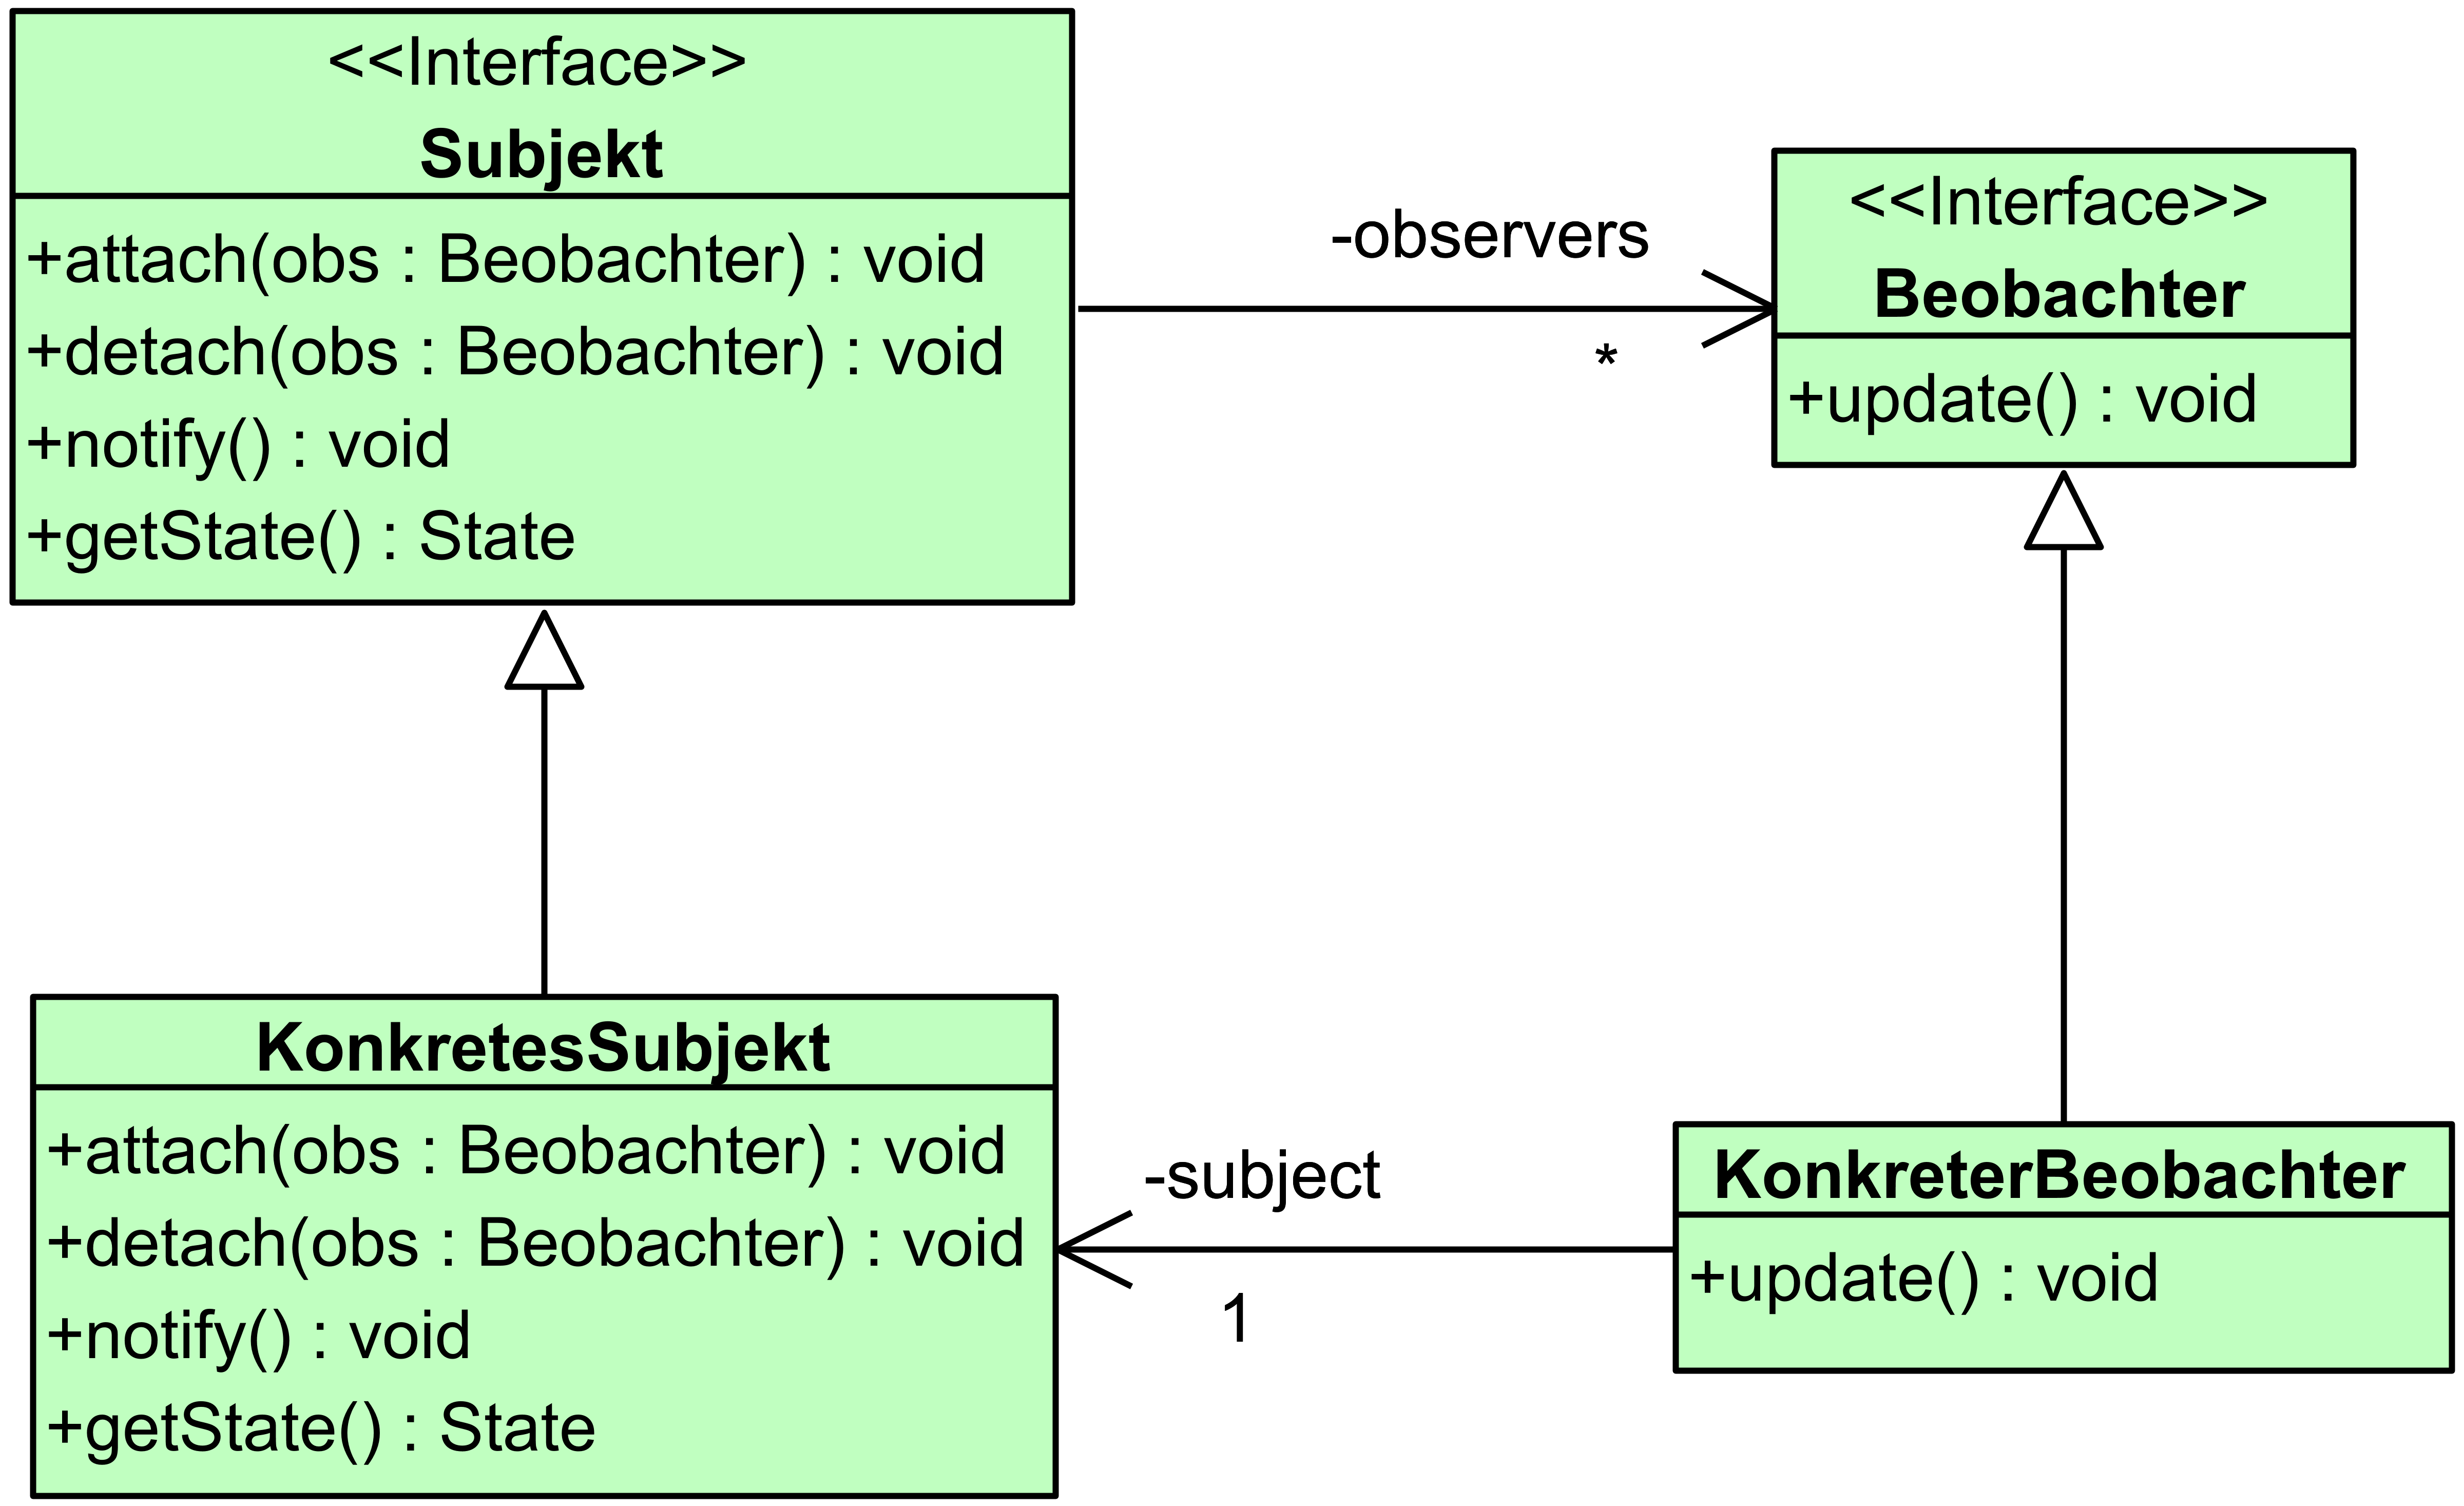
\includegraphics[width=\textwidth]{Abbildungen/Observer Pattern.png}
	\caption{UML-Diagramm -- Beobachter-Entwurfsmuster}
	\label{fig:observer_pattern}
\end{figure}
\noindent Das Entwurfsmuster benötigt für die korrekte Implementierung mindestens vier Komponenten (siehe \autoref{fig:observer_pattern}) \cite{Gamma1993}:
\begin{description}
	\item Das \texttt{\textbf{Subjekt}}, ist das zu beobachtende Objekt, welches zu jedem Zeitpunkt alle seine Beobachter in einer internen Datenstruktur speichert. Es besitzt Methoden zum An- und Abmelden von Beobachtern und ist in der Lage alle Beobachter bei eventuellen Zustandsänderungen zu benachrichtigen.
	\item Der \texttt{\textbf{Beobachter}} bietet eine Schnittstelle für Objekte, welche bei einer Zustandsänderung des Subjekts informiert werden sollen.
	\item Die \texttt{\textbf{KonkretesSubjekt}} Komponente ist die konkrete Implementierung der Subjekt Schnittstelle und ist fähig, einen internen Zustand zu verwalten, sowie bei einer Änderung von diesem, alle registrierten Beobachter zu informieren.
	\item Ein \texttt{\textbf{KonkreterBeobachter}} besitzt eine Referenz auf das zu beobachtende Subjekt und seinen internen Zustand. Bei einer Aktualisierung des Subjektzustands, wird auch der interne Zustand des konkreten Beobachters aktualisiert.
\end{description}
\subsection{MVC}
Das \ac{mvc} Entwurfsmuster ist ein de facto Standard der objektorientierten Programmierung \cite{Deacon1995}, welches für eine Trennung von grafischer Oberfläche, Eingaben des Benutzers und dem eigentlichen Anwendungsmodell sorgt \cite{Burbeck1992}. Hält eine Anwendung diese strikte Trennung ein, so genügt sie dem softwaretechnischen \ac{soc} Prinzip \cite{Grant2014}, woraus wiederum der Wartungsprozess vereinfacht und die Testbarkeit erhöht wird.
\begin{figure}[H]
	\centering
	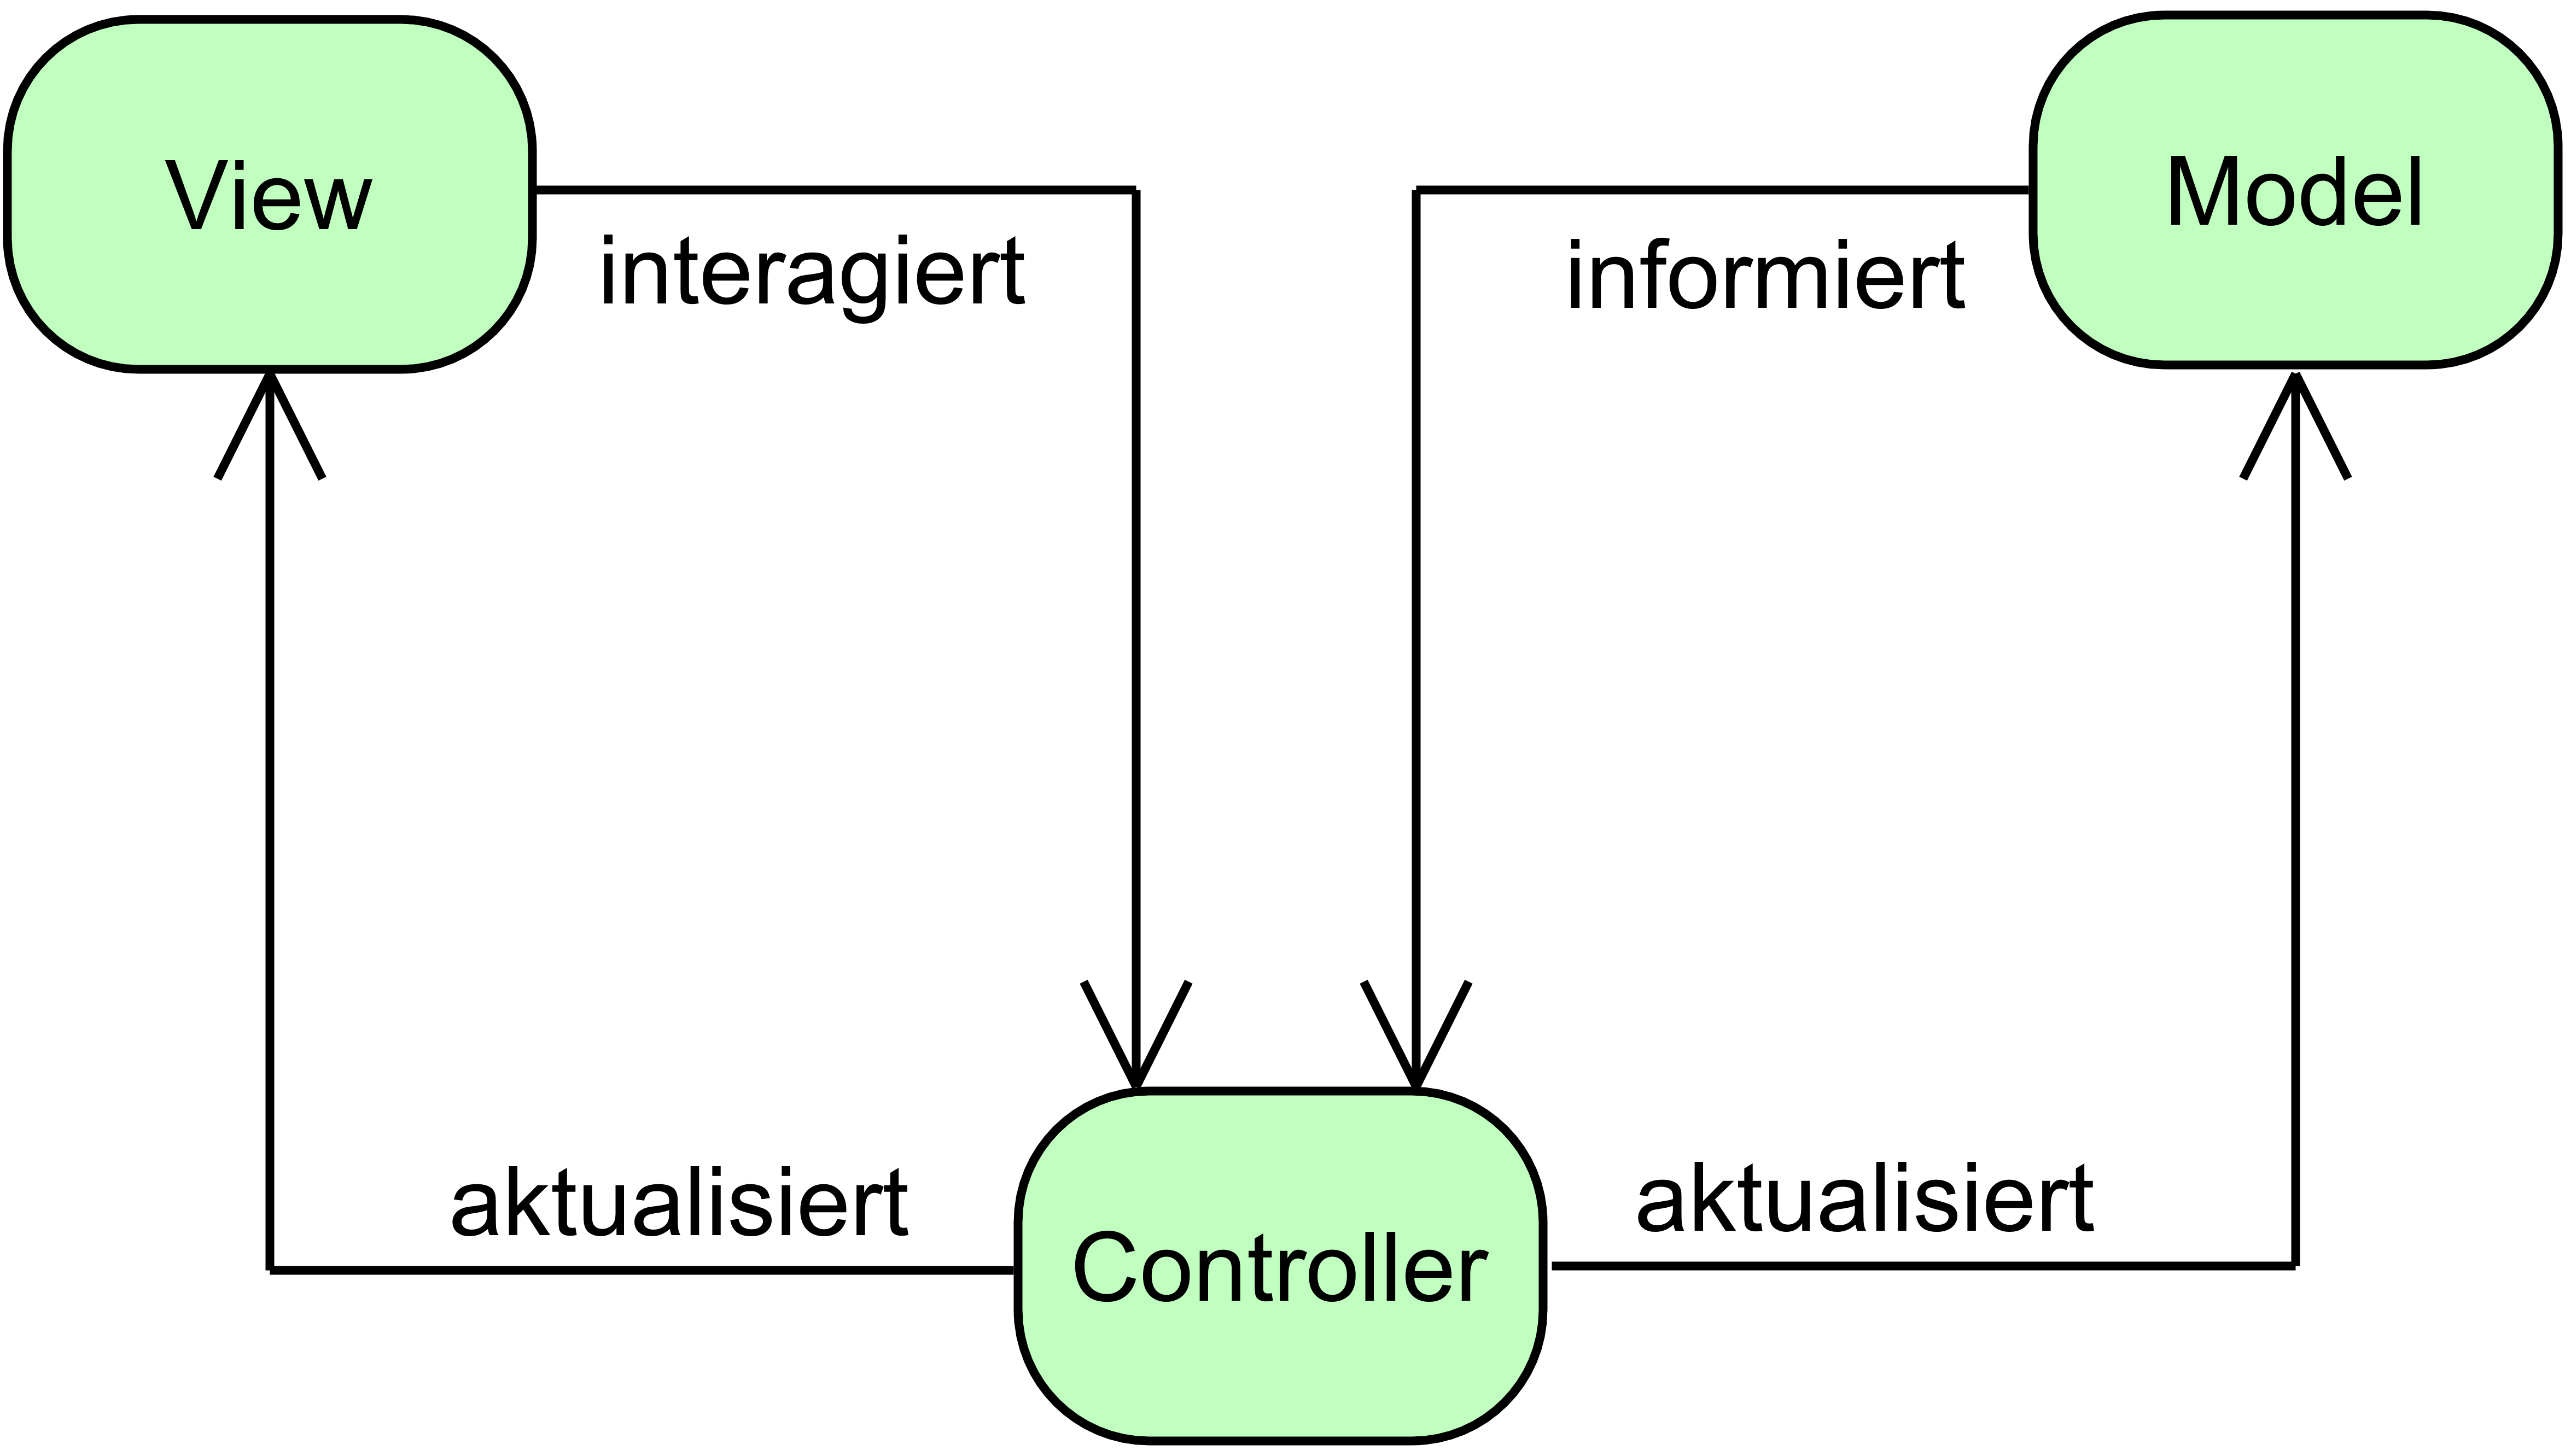
\includegraphics[width=\textwidth-2cm]{Abbildungen/MVC Pattern.png}
	\caption{Diagramm -- MVC-Entwurfsmuster}
	\label{fig:mvc_pattern}
\end{figure}
\noindent Die vom \ac{mvc} Muster vorgegebene Struktur ist, wie in \autoref{fig:mvc_pattern} zu sehen, in drei Komponenten unterteilt \cite{Deacon1995}:
\begin{description}
	\item Das \texttt{\textbf{Model}} beinhaltet alle Klassen welche für die Logik und die Datenhaltung der Anwendung verantwortlich sind und ist vollständig unabhängig vom View.
	\item Der \texttt{\textbf{View}} stellt die Anwendung dar, ermöglicht eine Interaktion mit diesem und ist in den meisten Applikationen äquivalent zu einer grafischen Benutzeroberfläche.
	\item Der \texttt{\textbf{Controller}} ist für das Verändern des Views verantwortlich. So werden beispielsweise Interaktionen mit der Benutzeroberfläche wie ein Schaltflächenklick im Controller verarbeitet, was wiederum den View aktualisiert. Der View und das Model sind vollständig entkoppelt und der Controller ist die Schnittstelle zwischen diesen.
\end{description}
\section{JavaFX}
\label{javafx}
\noindent JavaFX ist eine auf Java basierte, quelloffene Bibliothek für das Entwickeln von grafischen Benutzerschnittstellen für Client Applikationen. Im Vergleich zum Vorgänger GUI-Toolkit Java-Swing, bietet JavaFX ein modernes, zeitgemäßes Design der allgemeinen Benutzeroberfläche sowie den dort enthaltenen Schaltflächen und Komponenten \cite{Sharan2015}. Kombiniert mit den objektorientierten Konzepten von Java, ist JavaFX in der Lage auch komplexe nebenläufige Anwendungen mit vielen Abhängigkeiten darzustellen und aufgrund der Plattformunabhängigkeit auch ohne viele Restriktionen in allen bekannten Betriebssystemen einsetzbar.\\
Dazu ist JavaFX auch weitgehend konform mit bekannten Entwurfsmustern der Softwareentwicklung wie beispielsweise dem \ac{mvc}- oder dem Beobachter-Muster, weshalb implementierte Anwendung selbst bei vielen \ac{loc}, eine grundsätzlich hohe Strukturiertheit auf Quelltextebene aufweisen. Das grafische Layout kann dabei nicht ausschließlich durch Java-Quelltext sondern auch mittels der an die \ac{xml} angelehnte Markup-Sprache FXML erstellt werden. Letzteres kann durch externe Tools wie dem Scene-Builder enorm vereinfacht werden \cite{Vos2018}.

\subsection{Aufbau und Szenengraph}
\label{javafx_szenengraph}
Damit eine JavaFX-Anwendung als solche identifiziert werden kann, muss die Hauptklasse von der \texttt{Application}-Klasse erben. Die Namensgebung der Klassen, welche für die Struktur bzw. den Aufbau einer JavaFX-Anwendung zuständig sind, basiert auf Begriffe der Theaterumgebung \cite{Anderson2019}:
\begin{description}
	\item Die \textbf{\texttt{Stage}} Klasse repräsentiert ein Anwendungsfenster, welches das Design des Fensterlayouts des aktuell genutzten Betriebssystems nutzt. Eine \texttt{Stage} ist teilweise modifizierbar, so können beispielsweise die Standardschaltflächen in der Titelleiste entfernt order deaktiviert werden. Werden mehrere Fenster benötigt, so können nach dem Initialisieren der Haupt-\texttt{Stage} durch die JavaFX-Plattform, manuell Weitere hinzugefügt werden.
	\item Die \textbf{\texttt{Scene}} Klasse ist für das Layout und die Darstellung von vorhandenen oder selbsterstellten JavaFX-Komponenten verantwortlich. Jede Komponente, welche durch eine \texttt{Scene}-Instanz angezeigt und verwaltet werden soll, wird in einer hierarchisch angeordneten, objektorientierten Datenstruktur eingefügt, welche in der Computergrafik als Szenengraph bekannt ist \cite{Hughes2013}. Jeder \texttt{Stage} muss zwangsläufig eine \texttt{Scene} zugewiesen werden.
	\item Die \textbf{\texttt{Node}} Klasse ist eine darstellbare Komponente im Szenengraphen wie beispielsweise eine Schaltfläche oder ein Containerelement. \texttt{Node} Instanzen im Szenengraph können Kindelemente enthalten und maximal einem Elternelement zugeordnet sein. Der Szenengraph ähnelt somit einer Baumstruktur mit einer Wurzel und einem oder mehreren Blättern. Damit eine \texttt{Node}-Instanz Kindelemente besitzen darf, muss diese immer von der abstrakten \texttt{Parent}-Klasse erben. Das Layouting und die Positionierung im lokalen Koordinatensystem wird bei vorhandenen Kindelementen immer durch das Elternelement kontrolliert. Jede darzustellende Komponente muss von der \texttt{Node}-Klasse erben \cite{Juneau2013}.
\end{description}
Ein minimales Beispiel für eine voll funktionsfähige JavaFX-Anwendung, welche das Zusammenspiel der oben genannten Konzepte und Klassen widerspiegelt, ist in \autoref{lst:example_javafxapp} dargestellt.
\add{maybe beautify with fancy arrows}
\begin{figure}[H]
	\begin{lstlisting}[caption={Beispiel -- Minimale JavaFX-Anwendung.}, captionpos=b, label=lst:example_javafxapp]
		public class TestApplication extends Application {
			
			public static void main(String[] args) {
				Application.launch(args);
			}
			
			@Override
			public void start(Stage primaryStage) {
				final Pane root = new Pane();
				root.getChildren().add(new Button("TestButton"));
				final Scene scene = new Scene(root, 250, 250);
				primaryStage.setScene(scene);
				primaryStage.show();
			}
		
		}
	\end{lstlisting}
\end{figure}
\subsection{Properties und Bindings}
JavaFX besitzt eine auf dem JavaBeans-System und dem Observer-Entwurfsmuster basierende API, welche es dem Programmierer ermöglicht, eine synchronisierende Beziehung zwischen zwei oder mehr Variablen zu erstellen. Wird eine Variable in einer solchen Beziehung geändert, so wird automatisch auch die Andere geändert \cite{Hommel2013}. Dabei ist es auch möglich, Event Listener für eigene oder durch von JavaFX-Nodes automatisch erzeugte Properties zu registrieren. Soll beispielsweise Quelltext ausgeführt werden, wenn eine Änderung eines Wertes einer Property festgestellt wird, so kann dies mit dem Erstellen einer \texttt{ChangeListener}-Instanz durchgeführt werden \cite{Gao2019}. 
\begin{figure}[H]
	\begin{lstlisting}[caption=Beispiel -- ChangeListener \& EventHandler., captionpos=b, label=lst:property_example]
	Button btn = new Button("Test");
	// ChangeListener für den Schaltflächentext
	btn.textProperty().addListener((obs, oVal, nVal) -> {
	System.out.println(nVal);
	});	
	// EventHandler für die Schaltflächenaktivierung
	btn.setOnAction(e -> {
	System.out.println("Clicked!");
	})
	\end{lstlisting}
\end{figure}
\noindent Im ersten Teil von \autoref{lst:property_example} soll der Text einer Schaltfläche bei einer Änderung auf die Konsole ausgegeben werden. Dazu wird mittels Lambda Ausdruck ein neuer \texttt{ChangeListener} mit der \texttt{StringProperty} der Schaltfläche verknüpft.\\
Des Weiteren unterstützt JavaFX ein Event-System, welches anhand von verschiedenen Aktionen Events durch den Szenengraphen propagiert. Ein solches Event wird beispielsweise durch das Eintragen von Text in ein Textfeld oder das Aktivieren einer Dropdown-Liste ausgelöst. In zweiten Teil von \autoref{lst:property_example} wird ein \texttt{EventHandler} für das Aktivieren einer Schaltfläche erstellt.

\subsection{Layouting: FXML vs. Quelltext}
Wie in der Einleitung schon angedeutet, ist es möglich das Layout der Anwendung auch per FXML zu erstellen. Eine Prävention von Boilerplate-Code kann durch das Auslagern von häufig verwendeten JavaFX-Komponenten in externe FXML-Dateien erfolgen \cite{Kruk2018}. Das Verwenden von solchen Dateien sorgt für eine bessere Trennung von Controllern und Logik im Sinne des z.B. \ac{mvc}-Entwurfsmusters \cite{Juneau2013} und durch die hohe Konfigurierbarkeit sind für eine eventuelle Veröffentlichung der Applikation wichtige Konzepte wie die Internationalisierung, leichter umzusetzen \cite{Steyer2014}. Durch das Parsen und Aufbauen des Szenengraphen zur Laufzeit des Programms ist eine Verwendung von FXML-Dateien jedoch langsamer als benötigte Komponenten direkt im Java Quelltext zu deklarieren. Fast alle JavaFX-Nodes können ohne Weiteres in XML-Elementen verwendet und angepasst werden. Außerdem ist es möglich, direkt eine manuell erstellte Controller-Klasse mit einer FXML-Datei zu assoziieren. Das Laden einer FXML-Datei und das darauffolgende Aufbauen des Szenengraphen wird durch die \texttt{FXMLLoader}-Klasse durchgeführt. Das Layouting-Beispiel aus \autoref{lst:example_javafxapp} ist als eine funktionsgleiche FXML Variante in \autoref{lst:example_fxmllayouting} zu erkennen. Das Laden der Datei wird durch das Instanziieren eines neuen \texttt{FXMLLoader} Objekts, wie in \autoref{lst:example_fxmlloading} dargestellt, ermöglicht.

\begin{figure}[H]
	\begin{lstlisting}[caption={Beispiel -- FXML Layouting.}, captionpos=b, label=lst:example_fxmllayouting, language=XML]
	<?xml version="1.0" encoding="UTF-8"?>
	
	<?import javafx.scene.layout.Pane?>
	<?import javafx.scene.control.Button?>
	
	<Pane xmlns="http://javafx.com/javafx">
		<Button>TestButton</Button>
	</Pane>
	\end{lstlisting}
\end{figure}
\begin{figure}[H]
	\begin{lstlisting}[caption={Beispiel -- FXML Ladeprozess.}, captionpos=b, label=lst:example_fxmlloading]
Pane load(String fxmlPath) throws IOException {
	return new FXMLLoader(getClass().getResource(fxmlPath)).load();
}
	\end{lstlisting}
\end{figure}
\noindent Um eine Controller-Klasse mit der FXML-Datei zu assozieren, kann Wurzelelement dieser durch das \texttt{fx:controller} Attribut erweitert werden. Der Name des Controllers ist hierbei der voll qualifizierte Klassenname. Neben externen FXML-Dateien können auch externe \ac{css}-Dateien für das Design des Layouts verwendet werden. In \autoref{appendix:controllerbased_javafx_application} ist ein vollständig kompilierbares JavaFX-Programm welches aus einem Controller, einer FXML-Datei sowie einer CSS-Datei aufgebaut ist zu finden.
\section{Java-Annotationen}
\label{java_annotationen}
\noindent Annotationen sind in der Sprachwissenschaft eine Möglichkeit einen vorhandenen Text mit Anmerkungen zu versehen für beispielsweise Disambiguierung, also das Eliminieren von Mehrdeutichkeiten eines Wortes oder für das Erklären von komplexen Textabschnitten. Sie geben dem Leser Zusatzinformationen um Sachverhalte einfacher darzustellen und sorgen dadurch für ein schnelleres bzw. besseres Verständnis des Textes. Dabei sind solche Anmerkungen kein Hauptbestandteil von Texten sondern dienen ausschließlich als Ergänzung.\\
In der Informatik sind Annotationen ebenfalls nur ein deskriptives Strukturkonzept, welche es dem Entwickler ermöglicht, verschiedenen strukturellen Elementen der Programmierung (wie Felder oder Klassen), Metadaten zuzuweisen \cite{Yu2019}. Das Nutzen von Annotationen in Anwendungen ist aufgrund ihrer meist simpel gehaltenen Syntax auch für Programmiereinsteiger vorteilhaft und durch ihre Anpassungsfähigkeit und Flexibilität sind sie in vielen Bibliotheken und Programmiersprachen vertreten.
\subsection{Definition}
\label{java_annotationen_definition}
\add{Move footnote to first occurence}
\noindent Annotationen \footnote{Wenn in der Arbeit über Annotationen gesprochen wird, ist immer von Java-Annotationen auszugehen (außer anders angegeben)} wurden mit Java 5 (2014) in die Sprache eingeführt und werden seitdem immer häufiger für verschiedene Aspekte der Programmierung genutzt \cite{Rocha2011}. Mit ihnen kann eine Steuerung des Compilers erfolgen, eine Verarbeitung der Metadaten zu Kompilierzeit durchgeführt werden oder das Verhalten von Anwendungen zu Laufzeit modifiziert oder gelenkt werden \cite{Yu2019}. Aufgrund der Tatsache, dass es sich nur um rein deskriptive Metadaten handelt, ist es Annotationen nicht direkt möglich mit existierendem Quelltext zu interagieren.  Möglichkeiten zur Verarbeitung dieser Metadaten werden in Sektion \ref{java_annotation_laufzeitauswertung} vorgestellt. Neben den von Java vordefinierten Annotationen wie z.B. \texttt{@Override} für das Überschreiben von vererbten Methoden oder \texttt{@SuppressWarnings} für das Unterdrücken von Compilerwarnungen, können auch eigene Annotationen deklariert werden.\\
Es handelt sich bei Annotationen in Java um spezialisierte Schnittstellen bei welchen das \texttt{interface}-Schlüsselwort durch ein \texttt{@}-Zeichen Präfix zu \texttt{@interface} erweitert wird \cite{Gosling2005}. Außerdem ist es Annotationen nicht erlaubt wie bei normalen Schnittstellendefinitionen das Schlüsselwort \texttt{extends} für eine Vererbung zu verwenden, da die Superschnittstelle implizit vom Compiler auf die \texttt{Annotation} Klasse des \texttt{java.lang.annotation} Pakets gesetzt wird \cite{Oracle2017}. Ein Beispiel einer  Annotationsdefinition ist in \autoref{lst:annotation_definition} dargestellt.
\begin{figure}[H]
	\centering
	\begin{lstlisting}[caption={Beispiel einer Annotationsdefinition.}, captionpos=b, label=lst:annotation_definition]
	public @interface TestAnnotation {
	    // ...
	}
	\end{lstlisting}
\end{figure}
\noindent In der Analogie des Kapitels \ref{java_annotationen} können Elemente mit strukturgebenden Charakter wie Bestandteile eines Satzes annotiert werden. Analog dazu sind in der Java-Programmierung Klassen, Methoden, Felder etc. für die Strukturierung des Quelltextes und der Softwarearchitektur verantwortlich und somit auch mit Annotationen erweiterbar. Um Sprachelemente zu annotieren muss wie in \autoref{lst:annotated_example} dargestellt, ein \texttt{@}-Präfix zum eigentlichen Klassennamen hinzugefügt werden.
\begin{figure}[H]
	\centering
	\begin{lstlisting}[caption={Beispiel einer annotierten Klasse.}, captionpos=b, label=lst:annotated_example]
	#@TestAnnotation
	public class TestClass {
	    // ...
	}
	\end{lstlisting}
\end{figure}
\noindent Aufgrund der besonders einfachen Syntax und dem vergleichsweise geringen Aufwand, ist ein steigender Trend der Nutzung von Java-Annotationen in Open-Source Anwendungen zu erkennen. Werden Annotationen jedoch übermäßig verwendet, so kann es schnell zu Quelltext-Verschmutzung kommen, was im Kontext der Annotationsprogrammierung auch \glqq annotation hell\grqq{} (dt. Annotationshölle) genannt wird. Annotationen erreichen dann das Gegenteil des gewünschten Zwecks -- Statt den Entwicklungsprozess vereinfachend zu unterstützen, wird der Quelltext schwer nachvollziehbar und wirkt unstrukturiert und unübersichtlich.\\
Dennoch zeigt eine Studie aus dem Jahre 2019, welche 1094 quelloffene GitHub-Projekte auf die Verwendung von Annotationen untersucht hat, dass javabasierte Anwendungen und Bibliotheken, bei aktiver Nutzung von Annotationen, eine geringere Fehleranfälligkeit aufweisen \cite{Yu2019}.
\subsection{Syntax}
\label{java_annotationen_anwendung}
\add{lst design}
\addchap{use lstnewenvironment}
\noindent Annotationen können Attribute besitzen, welche bei Kompilierzeit bzw. Laufzeit ausgelesen werden können. Die Typen dieser Attribute sind nicht vollständig frei wählbar -- So ist es beispielsweise nicht möglich ein Attribut vom Typen \texttt{Object} in einer Annotation zu kapseln, ohne einen Kompilierfehler auszulösen. Erlaubt sind alle primitiven bzw. atomaren Datentypen und Instanzen der \texttt{String}-, \texttt{Class}- und \texttt{Enum}-Klasse sowie eindimensionale Arrays aus den vorherigen Typen. Außerdem ist es möglich, Attributen einen voreingestellten Wert mittels des Schlüsselwortes \texttt{default} zuzuweisen \cite{Gosling2005}. Annotationen müssen in einer der folgenden Syntaxen benutzt werden:
\begin{description}
	\item \textbf{Normal Annotations} sind ganz normal deklarierte Annotationen, bei welchen die Attribute mittels Aufzählung in Klammern übergeben werden.
	\begin{figure}[H]
		\noindent
		\newlength\heightone
		\begin{adjustbox}{minipage=[t]{.45\linewidth},gstore totalheight=\heightone,margin=\fboxsep+\fboxrule}
			\begin{lstlisting}[caption=Deklaration -- Normal Annotation., captionpos=b, label=lst:decl_normal]
public @interface Entity {
	String name();
	int id();
}
			\end{lstlisting}
		\end{adjustbox}\hfill
		\begin{adjustbox}{minipage=[t][\heightone]{0.5\linewidth}}
			\begin{lstlisting}[caption=Anwendung -- Normal Annotation, captionpos=b, label=lst:appl_normal]
#@Entity(name="test", id=2)
public class TestEntity {
	// ...
}
			\end{lstlisting}
		\end{adjustbox}
	\end{figure}
	\item \textbf{Single-Element Annotations} sind eine Kurzform der normalen Annotationen mit einem \texttt{value}-Attribut und keinen weiteren nicht-default Attributen.
	\begin{figure}[H]
		\noindent
		\begin{adjustbox}{minipage=[t]{.45\linewidth},gstore totalheight=\heightone,margin=\fboxsep+\fboxrule}
			\begin{lstlisting}[caption=Deklaration -- Single-Element Annotation., captionpos=b, label=lst:decl_single]
public @interface Entity {
	String value();
	int id() default -1;
}
			\end{lstlisting}
		\end{adjustbox}\hfill
		\begin{adjustbox}{minipage=[t][\heightone]{0.5\linewidth}}
			\begin{lstlisting}[caption=Anwendung -- Single-Element Annotation, captionpos=b, label=lst:appl_single]
#@Entity("test")
public class TestEntity {
	// ...
}
			\end{lstlisting}
		\end{adjustbox}
	\end{figure}
	\item \textbf{Marker Annotations} sind ebenfalls eine Kurzform der normalen Annotationen mit keinen oder nur default Attributen.
	\begin{figure}[H]
		\noindent
		\begin{adjustbox}{minipage=[t]{.45\linewidth},gstore totalheight=\heightone,margin=\fboxsep+\fboxrule}
			\begin{lstlisting}[caption=Deklaration -- Marker Annotation., captionpos=b, label=lst:decl_marker]
public @interface Entity {
	String name() default "";
	int id() default -1;
}
			\end{lstlisting}
		\end{adjustbox}\hfill
		\begin{adjustbox}{minipage=[t][\heightone]{0.5\linewidth}}
			\begin{lstlisting}[caption=Anwendung -- Marker Annotation, captionpos=b, label=lst:appl_marker]
#@Entity
public class TestEntity {
	// ...
}
			\end{lstlisting}
		\end{adjustbox}
	\end{figure}
\end{description}
\noindent Die Sichtbarkeit von eigenen Annotationen zu verschiedenen Phasen des Codezyklus kann durch die von Java bereitgestellte Annotation \texttt{@Retention} gesteuert werden. Das übergebene Enum-Attribut klassifiziert die Annotation dann in einen von drei Typen \cite{Rocha2011}:
\begin{description}
	\item \textbf{Quellcode-Annotationen} sind nur beim Kompiliervorgang auslesbar und können dem Compiler Anweisungen geben oder mithilfe von Annotation-Prozessoren z.B. neue Klassen automatisch generieren. Sie sind in der kompilierten Java-Anwendung nicht mehr erhalten.
	\item \textbf{Klassen-Annotationen} sind nach dem Kompilierungsprozess noch in der Anwendung erhalten und können durch externe Tools wie z.B. dem Code-Obfuskator ProGuard ausgelesen werden.
	\item \textbf{Laufzeit-Annotationen} sind nach der Kompilierung und beim Start der Anwendung erhalten und können dann mithilfe der Reflection-API zur Laufzeit ausgewertet werden.
\end{description}
\noindent Des Weiteren kann gesteuert werden, welche Typen der Strukturelemente eines Quellcodes annotiert werden können. Ein Beispiel für eine zur Laufzeit beibehaltene Annotation, welche nur an Methoden angebracht werden kann ist in \autoref{lst:full_annotation_example} zu erkennen.
\begin{figure}[H]
	\centering
	\begin{lstlisting}[caption={Beispiel einer Laufzeit Annotation.}, captionpos=b, label=lst:full_annotation_example]
	
	#@Target(ElementType.(@\tikzmark{aLeft}{}@)METHOD(@\tikzmark{aRight}{}@))
	#@Retention(RetentionPolicy.(@\tikzmark{bLeft}{}@)RUNTIME(@\tikzmark{bRight}{}@))
	public @interface Event {
		int id();
		int priority() default 0;
	}
	(@
	\begin{tikzpicture}[overlay,remember picture]
		\foreach \x/\y in {a/red, b/blue} {
			\DrawOverBar[-, \y, thick]{\x Left.north}{\x Right.north}
		}
		\node[draw](onlymethods) at (8.5,3) {Nur an Methoden};
		\node[draw](runtime) at (8.5,1.5) {Zur Laufzeit};
		\DrawArrow[red, in=-180]{a}{onlymethods}{-4.8em, 0}
		\DrawArrow[blue, in=-270, out=20]{b}{runtime}{0, 0.65em}
	\end{tikzpicture}
	@)
	\end{lstlisting}
\end{figure}

\add{Add compile time annotation processing if used in this thesis}
\subsection{Auswertung von Laufzeit-Annotationen}
\label{java_annotation_laufzeitauswertung}
Für eine Auswertung von Laufzeit-Annotationen, muss zwangsläufig die Reflection-API von Java genutzt werden. Wenn eine Programmiersprache eine Form von Reflection (dt. Spiegelung) aufweist, so ist es möglich Attribute, Logikfluss und andere Eigenschaften während der Laufzeit zu ändern. In objektorientierten Sprachen wie Java wird diese \glqq computational reflection\grqq{} genutzt, um die Möglichkeit einer Selbstbeobachtung der eigenen Sprachelemente zu schaffen \cite{Li2017}. Die API ermöglicht somit beispielsweise das Auslesen von Laufzeit-Annotationen und deren deklarierte Attribute oder das dynamische Instanziieren von Klassen \cite{Forman2004}. Jedes Java-Element der Reflection API (Feld, Methode, Klasse, ...), welches annotierbar ist, wird durch die Vererbung der \texttt{AnnotatedElement}-Klasse als solches klassifiziert \cite{Schildt2019}. Damit nun alle vorhandenen Annotation ausgelesen werden können, kann die Methode \inlinecode{java}{AnnotatedElement#getDeclaredAnnotations} aufgerufen werden \cite{Pigula2015}. Das Lesen der Attribute der in \autoref{lst:full_annotation_example} vordefinierten Annotation ist in \autoref{lst:annotation_processing_example} zu erkennen.
\begin{figure}[H]
	\begin{lstlisting}[caption={Auslesen einer Laufzeit-Annotation.}, captionpos=b, label=lst:annotation_processing_example]
    if(Test.class.isAnnotationPresent(Event.class)) {
	    Event e = Test.class.getDeclaredAnnotation(Event.class);
	    int id = e.id();
	    int priority = e.priority();
    }
	\end{lstlisting}
\end{figure}
\chapter{Stand der Technik}
\label{stand_der_technik}

\add{Intro}

\section{Aktuelle Verwendung von Annotationen}
\label{aktuelle_verwendung_von_annotationen}

\add{Intro}

\subsection{JavaFX}
\label{aktuelle_verwendung_von_annotationen_javafx}

\add{JavaFX Beispiele}

\subsection{Android}
\label{aktuelle_verwendung_von_annotationen_android}

\add{Android Beispiele}

\subsection{JavaX}
\label{aktuelle_verwendung_von_annotationen_javax}

\add{JavaX Beispiele (z.B. JAXB)}

\section{Maßnahmen zur Simplifizierung des Entwicklungsprozesses}
\label{maßnahmen_zur_simplifizierung_des_entwicklungsprozesses}

\add{Intro}

\subsection{Workflow Optimierung}
\label{maßnahmen_zur_simplifizierung_des_entwicklungsprozesses_workflow}

\add{Workflow Optimierung}

\subsection{Vereinfachung durch gesteigerte Übersichtlichkeit}
\label{maßnahmen_zur_simplifizierung_des_entwicklungsprozesses_übersichtichkeit}

\add{Vereinfachung durch gesteigerte Übersichtlichkeit}

\subsection{Fazit}
\label{maßnahmen_zur_simplifizierung_des_entwicklungsprozesses_fazit}

\add{Fazit}
\chapter{Konzeption und Entwurf}
\label{konzeption_und_entwurf}
In diesem Kapitel werden mögliche Probleme bei der Entwicklung sowie bei der Nutzung von JavaFX Anwendungen identifiziert. Dabei wird ein besonderer Fokus auf das Finden von Architekturmängeln, fehlenden Funktionalitäten und verbesserungswürdigen Techniken gelegt. Um eine Fehleranfälligkeit zu reduzieren, sollen komplexe und sich häufig wiederholende Quelltextbausteine automatisch erstellt oder durch Annotationen vereinfacht werden. Die vollständige Substitution eines aufwendige Prozesses ist dabei ebenfalls möglich. Probleme, Vereinfachungen oder Verbesserungen sollen durch das Untersuchen von vorhandenen, quelloffenen JavaFX-Projekten und Bibliotheken gefunden werden. Auch sollen Ideen und Konzepte zusammengetragen werden, welche auf JavaFX anwendbar sind, jedoch nur in anderen Bibliotheken und Frameworks aufzufinden sind. \\
Bei der Problemanalyse wird stets das Ziel verfolgt, das Entwickeln mit JavaFX zu vereinfachen -- besonders für noch unerfahrene Entwickler. Danach wird eine Anforderungsanalyse durchgeführt, mit welcher systematisch funktionale sowie nichtfunktionale Anforderungen auf der Basis der gefundenen Probleme erstellt werden. \\
Auf die Anforderungserhebung folgt die Konzeption des benötigten Systems und der zugrundeliegenden Architektur. Essentielle Komponenten werden mit \ac{uml} Diagrammen entworfen und im Detail erläutert. Bei der Existenz verschiedener Lösungsstrategien für ein Problem, wird jede Strategie einzeln beleuchtet und nach Kriterien wie Sinnhaftigkeit und Machbarkeit entschieden, welche für das System am besten geeignet ist. Wichtige Richtlinien wie die angestrebte Softwarequalität werden ebenfalls beschrieben.

\section{Identifikation von Problemen und komplexen Strukturen in der JavaFX Entwicklung}
\sectionmark{Identifikation von Problemen}
\label{problemanalyse}
Im Folgenden werden generelle Probleme bei der Entwicklung von JavaFX Anwendungen identifiziert. Dazu gehören Mechanismen welche aufgrund ihrer Komplexität nicht für Anfänger geeignet sind oder von erfahrenen Entwicklern häufig genutzt und somit möglicherweise vereinfacht werden können. Obwohl dabei Annotationen als Basis für eine Vereinfachung dienen, wird auch das Erstellen von zusätzlichen Klassen oder dem Entwickeln von Erweiterungen für existierenden JavaFX Konzepte als Alternative für diese Zielerreichung in Betracht gezogen. Die Lösungen der gefundenen Probleme werden in einer Anforderungsanalyse durch funktionale und nichtfunktionale Anforderungen in \autoref{anforderungsanalyse} gelöst.
\subsection{Internationalisierung und Lokalisierung}
In der Informatik, speziell in der Softwareentwicklung, ist die Internationalisierung ein wichtiger Bestandteil einen Softwareproduktes, bei welchen die Entwickler die Software so gestalten, dass diese ohne viel Aufwand für andere internationale Märkte mit anderen Kulturen und Sprachen verfügbar gemacht werden kann \cite{Reineke2005}. Dabei wird beispielsweise eine einfache Schnittstelle für das Verwenden von verschiedenen Sprachen entwickelt, welche das Übersetzen von vorhandenen Textfeldern und anderen textbasierte Elementen in grafischen Benutzeroberflächen, Konfigurationsdateien oder Konsolenausgaben ermöglicht. Die Schnittstelle wird dabei so entwickelt, dass ohne eine Änderung des Quelltextes, neue Sprachen hinzugefügt werden können. Die Lokalisierung beschreibt dann unter Anderem die Übersetzung von den eben genannten Elementen.\\
Dieses Konzept kann durch die von Java bereitgestellte \texttt{ResourceBundle} Klasse realisiert werden \cite{Deitsch2001}. Bei der Verwendung eines solchen \texttt{ResourceBundle}s wird jedem zu übersetzenden Element ein Schlüssel zugeordnet und nach Konvention, in einer \texttt{.properties} Datei gespeichert. Wenn eine neue Sprache im Laufe des Lokalisierungsprozesses hinzugefügt werden soll, so muss jeweils eine neue \texttt{.properties} Datei angelegt werden. JavaFX ermöglicht das manuelle Spezifizieren einer vordefinierten \texttt{ResourceBundle} Instanz bei dem Laden einer FXML Datei durch einen \texttt{FXMLLoader}.
In der zu ladenden FXML Datei müssen hartcodierte Textelemente durch den jeweiligen Schlüssel aus der \texttt{.properties} Datei, wie in \autoref{lst:fxmlkey} gezeigt, ersetzt werden.
\begin{figure}[H]
	\noindent
	\begin{adjustbox}{minipage=[t]{.45\linewidth},gstore totalheight=\heightone,margin=\fboxsep+\fboxrule}
		\begin{lstlisting}
## Properties Datei
login.user = Benutzername
		\end{lstlisting}
	\end{adjustbox}\hfill
	\begin{adjustbox}{minipage=[t][\heightone]{0.5\linewidth}}
		\begin{lstlisting}[language=XML]
<!-- FXML Datei -->
<Label text="%login.username"/>
		\end{lstlisting}
	\end{adjustbox}
	\captionof{lstlisting}{Nutzung des Schlüssels in einer FXML Datei.}
	\label{lst:fxmlkey}
\end{figure}
\noindent Das Problem bei dieser Art der Übersetzung ist, dass eine Änderung der Sprache zur Laufzeit des Programms nicht dynamisch möglich ist. Die FXML Datei bzw. der dazugehörige Controller muss nach einer Sprachänderung durch beispielsweise eine Schaltfläche oder ein Dropdown-Menü durch einen FXML-Loader neu geladen werden, damit eventuelle Änderungen übernommen werden können. Das dynamische Ändern der Sprache zur Laufzeit ist nur mit einem Modifizierung des Ladeprozesses von FXML Dateien durch eine eigene Version des \texttt{FXMLLoader}s oder durch eine vom \texttt{FXMLLoader} unabhängige Implementierung durch Properties und Bindings möglich. Die erste Variante sorgt für ein automatisches Binden der nötigen Properties und die Letztere für ein manuelles Binden wenn nötig, weshalb eine Fusion beider Möglichkeiten in eine hohe Anpassbarkeit des Systems resultiert. Außerdem ist es auf diese Weise möglich, verschiedene Bindings zu aktualisieren, falls ein bestimmtes Event auftritt, welches eine Änderung des übersetzten Textes hervorruft. Parameterisierte Schlüssel aus der \texttt{.properties} Datei können somit automatisch an die parameterverändernden Events gebunden werden.

\section{Anforderungsanalyse}
\label{anforderungsanalyse}
In der Anforderungsanalyse werden die gefundenen Problemlösungen und Vereinfachungen aus \autoref{problemanalyse} in Form von funktionalen und nichtfunktionalen Anforderungen formuliert. Dabei werden die Anforderungen in zwei Klassen unterteilt:
\begin{description}
	\item \textbf{Fundamentale Anforderungen} sind Anforderungen, welche für eine Funktion des Systems essentiell sind, alle genannten Probleme weitgehend beheben und daher zwangsläufig implementiert werden müssen.
	\item \textbf{Optionale Anforderungen} sind Anforderungen, welche keinen Einfluss auf eine ordnungsgemäße Funktionalität des Systems haben. Sie sind optional und werden möglicherweise aufgrund ihrer Komplexität nur teilweise oder gar nicht implementiert und können stattdessen für eine Erweiterung des Systems durch weitere Entwickler genutzt werden.
\end{description}
\add{format of requirements}

\subsection{Funktionale Anforderungen}
\label{anforderungsanalyse_funktional}
Im Folgenden werden alle funktionalen Anforderungen definiert. Sie beschreiben alle gewünschten Funktionen des Endproduktes.
\add{09.06}

\add{Funktionale Anforderungen als Unterpunkte}
\subsubsection{...}

\subsection{Nichtfunktionale Anforderungen}
\label{anforderungsanalyse_nichtfunktional}
Im Folgenden werden alle nichtfunktionalen Anforderungen definiert. Sie beschreiben Qualitätseigenschaften an das System wie Möglichkeiten der Erweiterbarkeit und Wartbarkeit und spezifizieren Maßstäbe, welche zur Laufzeit der Anwendung eingehalten werden müssen. Darunter gehören beispielsweise die effiziente Ressourcennutzung, die Korrektheit des Systems sowie ein gewisser Grad an Zuverlässigkeit.
\add{09.06}

\add{Nichtfunktionale Anforderungen als Unterpunkte}
\subsubsection{...}

\section{Konzept und Modellierung}
\label{konzept_und_modellierung}
\add{10.06-13.06}
\add{Intro}

\subsection{Designentscheidungen}
\label{konzept_und_modellierung_designentscheidungen}

\subsection{...}
\chapter{Implementierung}
\label{implementierung}
In diesem Kapitel werden wichtige Aspekte bei der Implementierung des Systems aufgezeigt. Auf essentielle Quelltextausschnitte, welche für eine Gewährleistung der, aus den Anforderungen resultierenden, Funktionalität verantwortlich sind, wird detailliert eingegangen. Dabei werden wichtige Konzepte, Strukturen und Designentscheidungen der entwickelten Architektur hervorgehoben und aufgetretene Probleme beim Implementierungsprozess dargelegt. Außerdem werden ausgewählte Subsysteme von \texttt{SimpliFX} mit geeigneten Darstellungsmitteln präsentiert und, für ein besseres Verständnis der zusammenarbeitenden Komponenten, eine beispielhafte Nutzung dieser durchgeführt. Die Verwendung und das Zusammenspiel der zuvor in \autoref{annotations} definierten Annotationen werden durch Quelltextbeispiele erklärt. Dazu werden mögliche mit einhergehende Restriktionen beleuchtet.
\section{Architektur und Struktur der Software}
\label{architektur}
Für die Implementierung und um eine, nach \autoref{nreq25} und \autoref{nreq26}, hohe Softwarequalität sowie Erweiterbarkeit zu ermöglichen, muss das System durch eine wohlüberlegte Architektur repräsentiert werden. Um eine hohe Unabhängigkeit des Systems zu gewährleisten und eine Überladung mit unnötigen Funktion zu vermeiden, wurde auf die Nutzung von externen Bibliotheken zur Vereinfachung des Implementierungsprozesses und die Reduktion des Zeitaufwandes weitgehend verzichtet. Nur externe Bibliotheken, welche komplexe Funktionen zur Verfügung stellen und daher nicht im Rahmen dieser Arbeit implementiert werden können, sind im Projekt enthalten. Auch dürfen Bibliotheken, welche eine Inkompatibilität mit der im Projekt genutzten Softwarelizenz aufweisen, nicht als Abhängigkeit genutzt werden. Für die Verwaltung der externen Bibliotheken und die Strukturierung des Systems wird, wie in \autoref{konzept_und_modellierung_designentscheidungen} erläutert, das Apache Maven\footref{ft:maven} Build-Management-Tool verwendet. Das Projekt wird nach der finalisierten Implementierung als Maven-Artefakt öffentlich zugänglich gemacht und aufgrund der quelloffenen Natur auch per GitHub einsehbar sein. \texttt{SimpliFX} bietet dem Nutzer dazu auch verschiedene spezialisierte Artefakte an, welche an ein bestimmtes Framework für die Abhängigkeitsinjektion angepasst wurden. Für die interne Trennung der Belange und Funktionen von \texttt{SimpliFX} werden Java Pakete verwendet. Diese Paketstruktur wird im nachfolgenden Unterkapitel näher erläutert. Dabei wird auf die Funktionalität der, in den einzelnen Paketen definierten, Klassen eingegangen und mögliche wichtige Funktionen, Methoden und Klassen mit Beispielen und ausgewählten Quelltextausschnitten vorgestellt und explizit angegeben, ob eventuelle Restriktionen bei der Nutzung zu beachten sind.
\section{Paketstrukturierung nach Funktionalität}
Die verschiedenen Pakete von \texttt{SimpliFX} sind in \autoref{fig:package_structure} dargestellt. Rot markierte Pakete dienen zur Abhängigkeitsinjektion und sind nicht im normalen Funktionsumfang enthalten, sondern nur mittels spezialisierter Maven-Artefakte nutzbar. 
\def\Size{4pt}
\definecolor{folderbackground}{RGB}{135,147,154}
\tikzset{
  folder/.pic={
    \filldraw[draw=folderbackground,top color=folderbackground!50,bottom color=folderbackground]
      (-1.05*\Size,0.2\Size+5pt) rectangle ++(.75*\Size,-0.2\Size-5pt);  
    \filldraw[draw=folderbackground,top color=folderbackground!50,bottom color=folderbackground]
      (-1.15*\Size,-0.7*\Size) rectangle (1.15*\Size,\Size);
  },
  folderopt/.pic={
    \filldraw[draw=red,top color=red!50,bottom color=red]
      (-1.05*\Size,0.2\Size+5pt) rectangle ++(.75*\Size,-0.2\Size-5pt);  
    \filldraw[draw=red,top color=red!50,bottom color=red]
      (-1.15*\Size,-0.7*\Size) rectangle (1.15*\Size,\Size);
  }
}
\begin{figure}[H]
	\centering
	\begin{forest}
		for tree={
			font=\ttfamily,
			grow'=0,
			child anchor=west,
			parent anchor=south,
			anchor=west,
			inner xsep=8pt,
			inner ysep=0pt,
			if n=6{edge path={\noexpand\path [draw, \forestoption{edge}] (!u.south west)+(12.5pt,0) |- (.child anchor) pic {folderopt}\forestoption{edge label};}}{if n={12}{edge path={\noexpand\path [draw, \forestoption{edge}] (!u.south west)+(12.5pt,0) |- (.child anchor) pic {folderopt}\forestoption{edge label};}}{if n={15}{edge path={\noexpand\path [draw, \forestoption{edge}] (!u.south west)+(12.5pt,0) |- (.child anchor) pic {folderopt}\forestoption{edge label};}}{edge path={\noexpand\path [draw, \forestoption{edge}] (!u.south west)+(12.5pt,0) |- (.child anchor) pic {folder}\forestoption{edge label};}}}},
			if n children=0{}{
				delay={
					prepend={[,phantom, calign with current]}
				}
			},
			fit=band,
			before computing xy={l=35pt}
		}
		[de.intelligence.bachelorarbeit.simplifx
			[application]
			[classpath]
			[config]
			[controller]
			[css]
			[dagger1]
			[di]
			[event]
			[events]
			[exception]
			[experimental]
			[fxml]
			[guice]
			[localization]
			[shared]
			[spring]
			[utils]
		]
	\end{forest}
	\caption{Paketstruktur -- \texttt{SimpliFX}}
	\label{fig:package_structure}
\end{figure}
\subsection{Paket: utils}
Das \texttt{utils} Paket beinhaltet Klassen und Methoden, welche häufig genutzte Operationen an zentraler Stelle kombiniert. Außerdem werden Werkzeugklassen bereitgestellt, die in der Form nicht im Funktionsumfang von Java enthalten sind. Dazu gehören beispielsweise funktionale Schnittstellen mit einer Unterstützung von Ausnahmen, Klassen für das Überprüfen von Nullbarkeit oder bool'schen Bedingungen und Implementierungen der \texttt{Iterator} Schnittstelle, welche durch das Nutzen von \texttt{AutoCloseable} Ressourcen schließen kann und damit eine Prävention von eventuellen Ressourcenlecks gewährleistet. Die Klasse \texttt{CloseableWrappedIterator} erlaubt das Erstellen einer \texttt{Iterator} Instanz, welche bei Nutzung der \texttt{stream} Methode alle genutzten Ressourcen bei einem Ende des Streams automatisch schließt. Außerdem wurde die Funktionalität der \texttt{Map.Entry} Klasse in die \texttt{Pair} Klasse ausgelagert, von welcher eine beispielhafte Nutzung in \autoref{lst:pair} dargestellt ist.
\begin{figure}[H]
	\begin{lstlisting}[caption=Beispiel -- Nutzung der \texttt{Pair} Klasse, captionpos=b, label=lst:pair]
final Pair<String, Integer> pair = Pair.of("test", 0);
System.out.println(pair.getLeft()); // test
System.out.println(pair.getRight()); // 0
	\end{lstlisting}
\end{figure}
\subsection{Paket: di}
\label{package_di}
Schnittstellen für die Unterstützung von Abhängigkeitsinjektion werden durch das \texttt{di} Paket bereitgestellt. Die eigentliche Implementierung dieser Schnittstellen ist in externen  Artefakten zu finden, auf welche in den folgenden drei Untersektionen näher eingegangen wird.
Das Paket stellt drei Klassen, \texttt{DIEnvironment} und \texttt{IDIEnvironmentFactory} sowie die \texttt{@DIAnnotation} zur Verfügung. Wenn eine weitere Bibliothek zur Laufzeitinjektion von Abhängigkeiten genutzt werden soll, welche nicht im Funktionsumfang von \texttt{SimpliFX} enthalten sind, müssen Implementationen für beide Schnittstellen, sowie eine Annotation für die jeweilige Bibliothek bereitgestellt werden.
\begin{figure}[H]
	\centering
	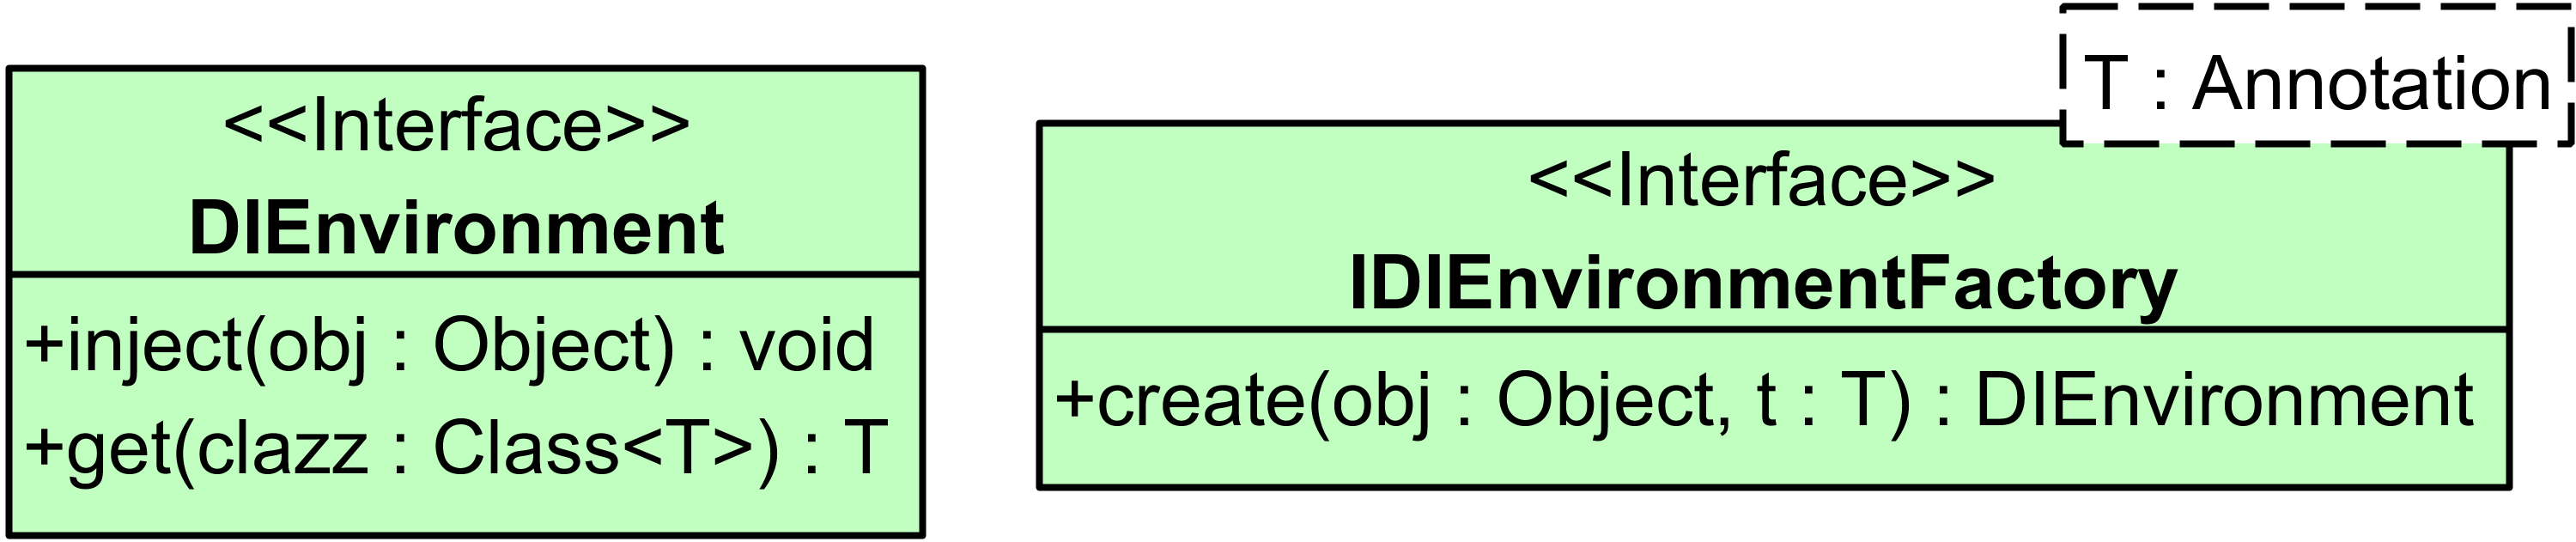
\includegraphics[width=\textwidth-2cm]{Abbildungen/DI Paket.png}
	\caption{Diagramm -- DI Schnittstellen}
	\label{fig:di_package}
\end{figure}
\noindent \texttt{SimpliFX} kennt die Implementierung der in \autoref{fig:di_package} dargestellten Klassen nicht und kann daher mit Leichtigkeit um weitere Bibliotheken zur Abhängigkeitsinjektion erweitert werden. Zuerst muss der Entwickler eine Implementierung der \texttt{DIEnvironment} Klasse erstellen, welche für das Injizieren von vorhandenen Objekten und das Instanziieren von neuen Objekten verantwortlich ist. Danach muss eine \texttt{IDIEnvironmentFactory} mit dem Typen der Annotation als generischen Parameter erstellt werden, welche den alleinigen Zweck hat, neue Instanzen der vorher erstellten \texttt{DIEnvironment} Implementierung zu generieren. Letztlich muss der Entwickler eine Laufzeitannotation erstellen, welche an Typdefinitionen angebracht werden kann und dazu die Meta-Annotation \texttt{@DIAnnotation} mit der jeweiligen Implementierungsklasse der \texttt{IDIEnvironmentFactory} Schnittstelle als Parameter aufweist. Das Registrieren einer neuen Bibliothek ist in \autoref{appendix:add_new_di_library} gezeigt.
\subsection{Paket: dagger1}
Das \texttt{dagger1} Paket ist für die Integration von Dagger 1\footnote{Dagger 2 realisiert Abhängigkeitsinjektion ausschließlich zur Kompilierzeit, weshalb Schnittstellen zum reflektiven Injizieren von Abhängigkeiten wie den \texttt{ObjectGraph} nicht mehr existieren und somit ein Zugang von \texttt{SimpliFX} auf den Injizierungsprozess ausgeschlossen ist.} in \texttt{SimpliFX} zuständig. Die \texttt{Dagger1Environment} Klasse definiert eine neue \texttt{ObjectGraph} Instanz aus den übergebenen Modulobjekten, welche für die Injektion verantwortlich ist. Dabei kann die Methode \texttt{ObjectGraph\#inject} genutzt werden, um Abhängigkeiten in eine vorhandene Instanz zu injizieren und \texttt{ObjectGraph\#get}, um eine neue Klasseninstanz zu erstellen. 
\subsection{Paket: guice}
Das \texttt{guice} Paket ist für die Integration von Guice in \texttt{SimpliFX} zuständig. Dabei wird von der \texttt{GuiceEnvironment} Klasse ein neuer \texttt{Injector} erstellt, welcher durch die Methode \texttt{Injector\#injectMembers} Abhängigkeiten injiziert und mit \texttt{Injector\#getInstance} neue Instanzen erstellt.
\subsection{Paket: spring}
Das \texttt{spring} Paket ist für die Integration von Spring in \texttt{SimpliFX} zuständig.
Die Umgebungsklasse für Spring (\texttt{SpringEnvironment}) erstellt eine neue Instanz der \texttt{AnnotationConfigApplicationContext} Klasse, welche es ermöglicht, mittels einer \texttt{AutowireCapableBeanFactory} Abhängigkeiten in bestehende Instanzen zu injizieren, sowie neue Instanzen aus Klassen zu erstellen.
\subsection{Paket: localization}
Alle Klassen und Funktionen, welche für das Umsetzen der dynamischen Lokalisierung benötigt wurden, sind im \texttt{localization} Paket enthalten. Dazu gehören beispielsweise die \texttt{II18N} Schnittstelle, eine Standard-Implementierung dieser und die \texttt{LocalizeValue} Annotation. 
\subsection{Paket: controller}
Das vollständige Controller-System ist im \texttt{controller} Paket enthalten. Das System kann auch unabhängig verwendet werden. Es ist jedoch ratsam, \texttt{SimpliFX} für die Initialisierung zu nutzen, da vorkonfigurierte Klassen wie beispielsweise \texttt{I18N} dafür benötigt werden. Das System kann durch die Erstellung eines neuen \texttt{IControllerGroup} Objektes gestartet werden. Die Schnittstelle stellt das Fundament des System dar und ist in \autoref{fig:controller_group_def} abgebildet. Durch die \texttt{start}-Methode kann die aktuelle Controllergruppe gestartet werden. Ist der Startcontroller zu dem Zeitpunkt noch nicht erstellt worden, so wird dieses mittels eines Aufruf der \texttt{constructController}-Methode nachgeholt. Diese Methode kann auch durch den Entwickler genutzt werden, um Controller zu generieren, bevor diese verwendet werden. Jede Gruppe muss exakt einen aktiven Controller besitzen, welcher durch \texttt{switchController} mit einer Standardanimation oder einer eigenen Animation gewechselt werden kann. Wird ein Controller bzw. eine Gruppe nicht weiter benötigt, so können mit den Aufruf der jeweiligen \texttt{destroy} Methode, alle gespeicherten Ressourcen und Instanzen gelöscht werden. Die von \texttt{SimpliFX} verwendete Implementierung dieser sowie eine Darstellung der verschiedenen Beziehungen zu anderen Komponenten des Systems ist in \autoref{appendix:controller_system} zu erkennen.
\begin{figure}[H]
	\centering
	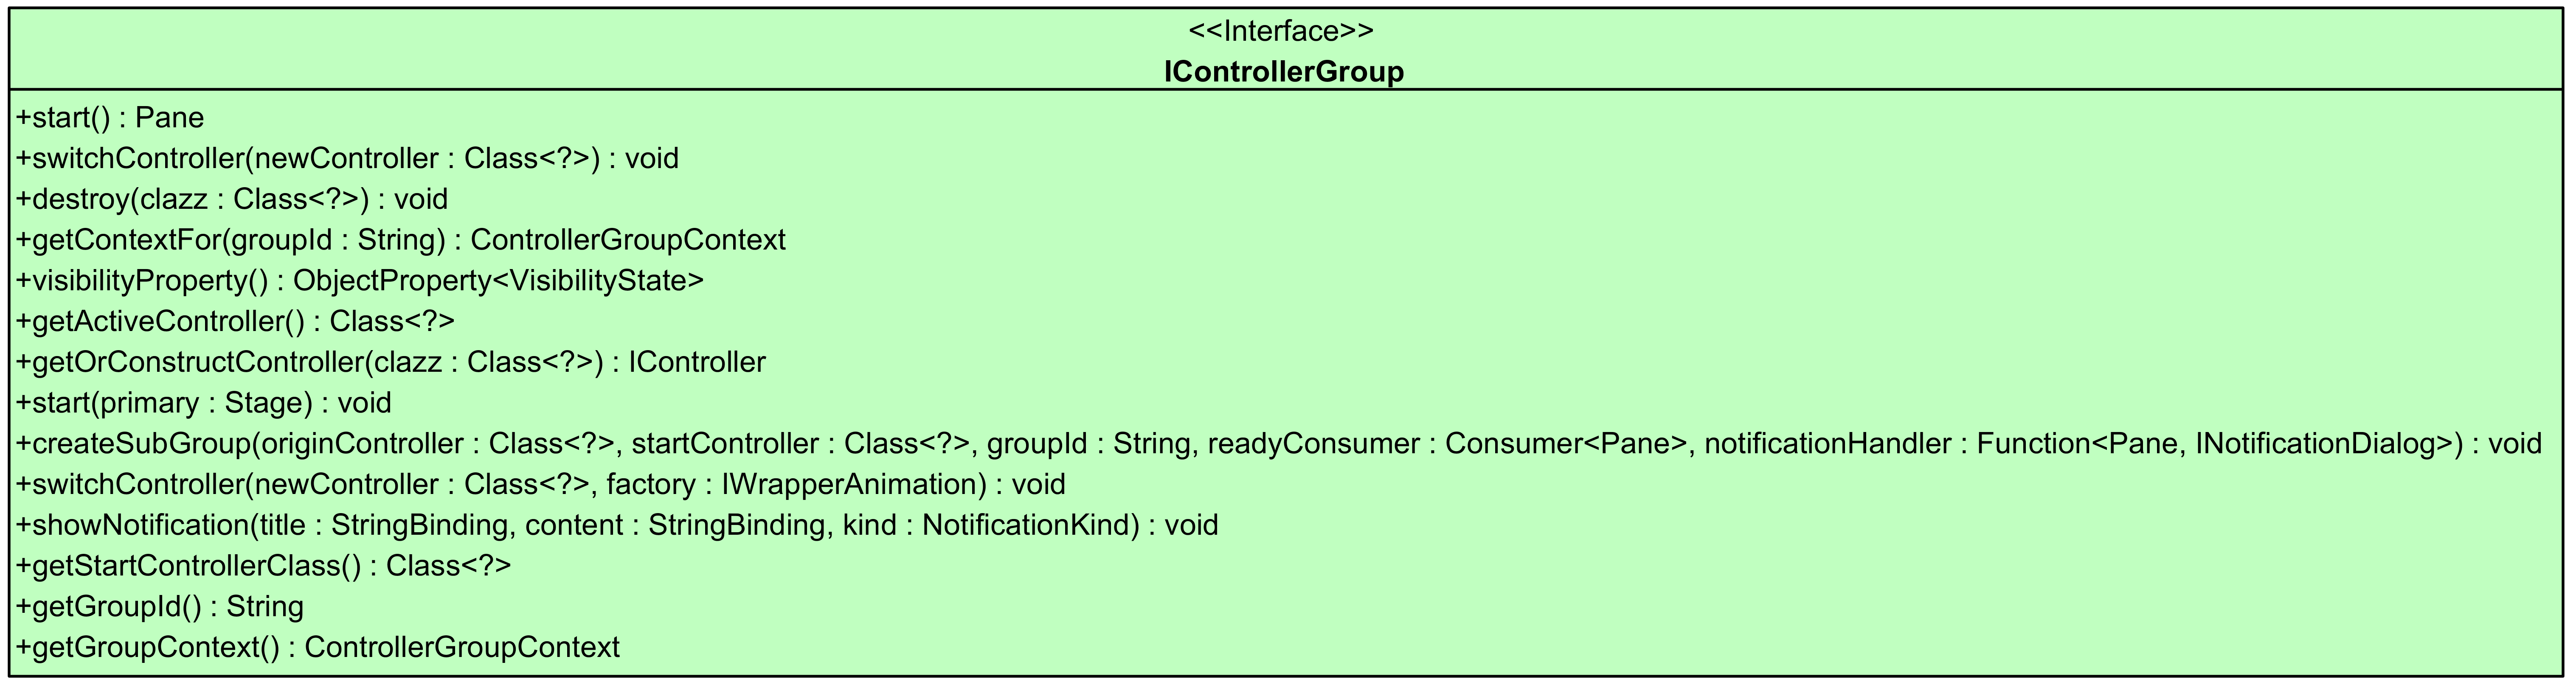
\includegraphics[width=\textwidth]{Abbildungen/Controller-System-Group.png}
	\caption{Diagramm -- Einstiegspunkt des Controller-Systems}
	\label{fig:controller_group_def}
\end{figure}
\noindent Controllergruppen werden anhand eines \texttt{String}s eindeutig identifiziert und bei Konstruktion in einer globalen \texttt{ControllerRegistry} registriert, um doppelte Identifikatoren zu vermeiden. Dazu werden Controllerklassen vor der Konstruktion validiert. So ist es beispielsweise nicht erlaubt, eine nicht-statische, innere Klasse als Controller zu
 definieren, da eine direkte Instanziierung der Klasse durch \texttt{SimpliFX} in diesem Fall ausgeschlossen ist.
\subsection{Paket: exception}
Eigene Ausnahmeklassen sind im \texttt{exception} Paket aufzufinden. Dazu gehören spezielle Ausnahmen für das Controller-System oder generelle Ausnahmen, welche von einer Vielzahl der \texttt{SimpliFX}-Komponenten genutzt werden.
\subsection{Paket: css}
Alle \ac{css} bezogenen Klassen sind im \texttt{css} Paket enthalten. Einige davon werden dabei ausschließlich durch den \texttt{SimpliFXMLLoader} genutzt, um automatisch \ac{css} Metadaten für eigene JavaFX-Komponenten zu generieren. 
\subsection{Paket: experimental}
Experimentelle Funktionen sind im \texttt{experimental} Paket zu finden. In der aktuellen Version der Bibliothek beinhaltet das Paket nur Klassen, welche für die Umsetzung der FX-Thread Forcierung (\autoref{freq21}) benötigt werden.
\subsection{Paket: classpath}
Wie bereits im Konzept beschrieben, wird für das Finden der Applikation- bzw. Preloader-Klasse ein System benötigt, welches in der Lage ist, den Klassenpfad zur Laufzeit des Programms nach Dateien zu durchsuchen. Dieses System findet nahezu alle Klassen und Ressourcen aus dem Klassenpfad, wird momentan aber nur für das Finden der jeweiligen Einstiegspunkte verwendet. Nur Klassenpfade aus einer unkomprimierten Orderstruktur (beispielsweise bei der Nutzung von verschiedenen Entwicklungsumgebungen) und aus komprimierten JAR-Archiven sind möglich. Die Architektur ermöglicht aber ein Hinzufügen von weiteren Klassenpfadquellen wie zum Beispiel WAR-Archiven (siehe \autoref{fig:classpath_sources}). 
\begin{figure}[H]
	\centering
	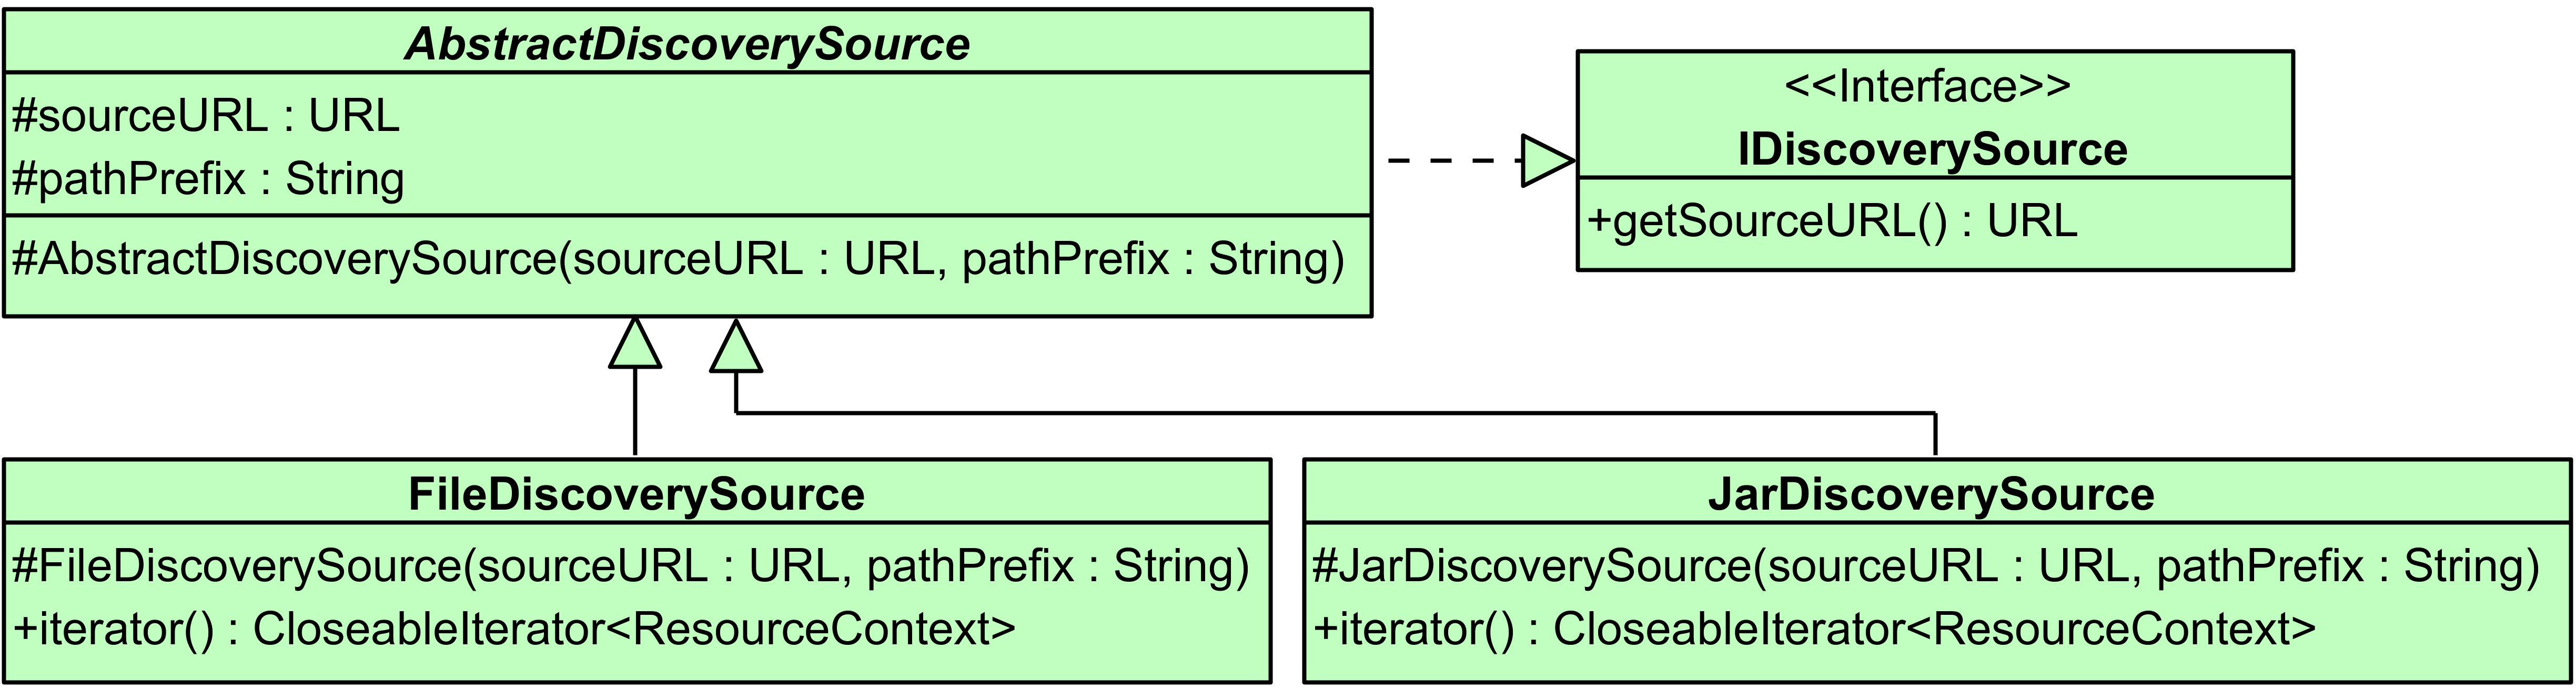
\includegraphics[width=\textwidth-2cm]{Abbildungen/Klassenpfadscan-Sources.png}
	\caption{Diagramm -- Mögliche Quellen für Klassenpfade}
	\label{fig:classpath_sources}
\end{figure}
\noindent Damit ein Klassenpfadscan initiiert werden kann, muss, wie in \autoref{fig:classpath_interface} dargestellt, eine neue Instanz der \texttt{ClassDiscovery} Klasse erstellt werden. Eventuelle Konfigurationen wie das Hinzufügen weiterer \texttt{ClassLoader} oder dem Spezifizieren eines Basispfades, welcher den zu scannenden Klassenpfad einschränkt und somit in den meisten Fällen zu einer Reduktion der benötigten Scanzeit beiträgt, können durch die Nutzung des \texttt{DiscoveryContextBuilder} erreicht werden. Der \texttt{DiscoveryContextBuilder} bietet dabei auch standardisierte Konfigurationen an.
\begin{figure}[H]
	\centering
	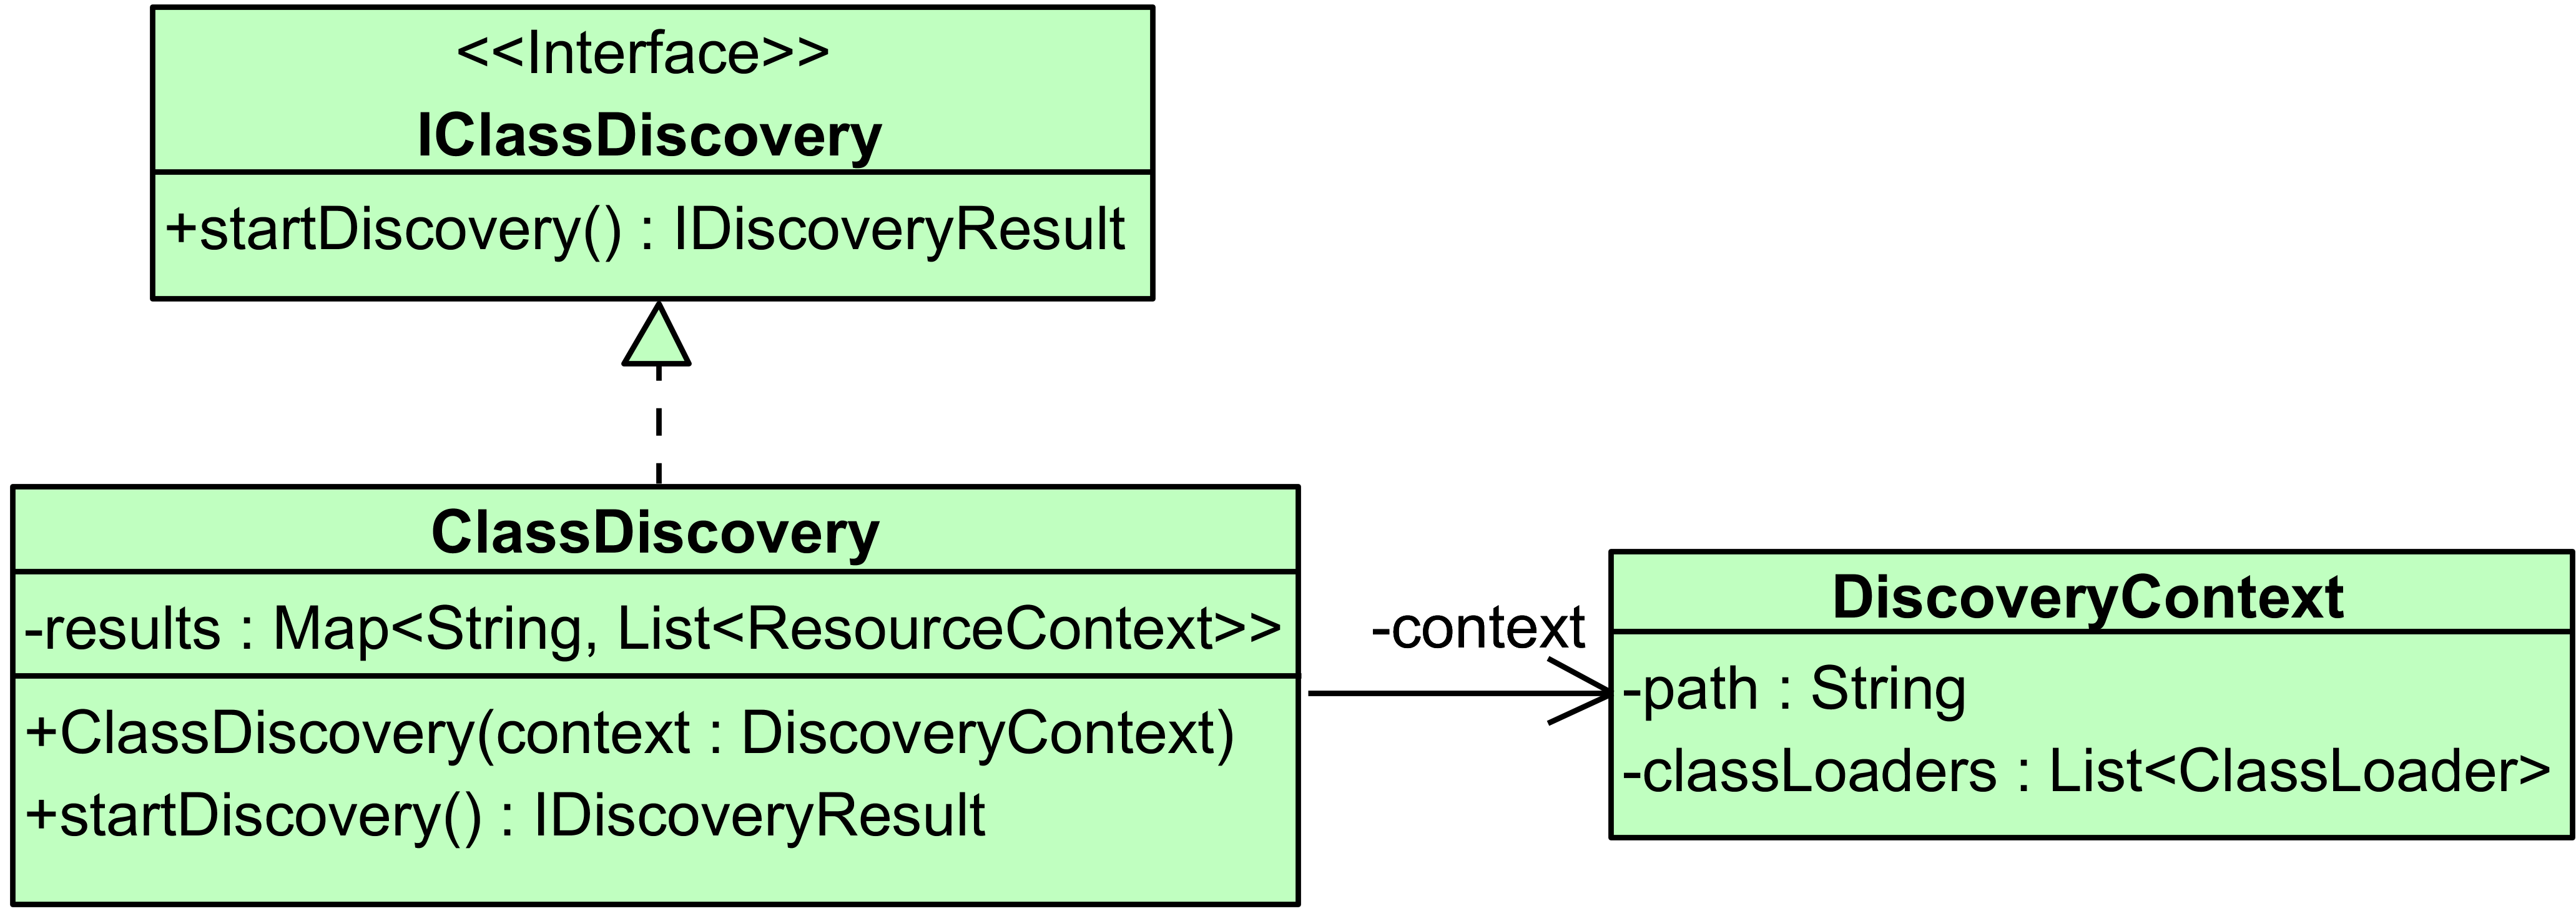
\includegraphics[width=\textwidth-2cm]{Abbildungen/Klassenpfadscan-Discovery.png}
	\caption{Diagramm -- Klassenpfad Schnittstelle und Implementierung}
	\label{fig:classpath_interface}
\end{figure}
\noindent Eine beispielhafte Nutzung des Klassenpfadscans ist im folgenden Quelltextausschnitt dargestellt:
\begin{figure}[H]
	\begin{lstlisting}[caption=Beispiel -- Initiierung eines Klassenpfadscans., captionpos=b, label=lst:classpath_scan_usage]
// Startet einen Scan mit Standardkonfiguration
var r = new ClassDiscovery(new DiscoveryContextBuilder()
		.setDefaultClassLoaders().build()).startDiscovery());
// Sucht alle mit @StageConfig annotierten Klassen
List<Class<?>> a = r.findClassesAnnotatedBy(StageConfig.class);
	\end{lstlisting}
\end{figure}
\subsection{Paket: shared}
Die für das Konzept der geteilten Ressourcen benötigten Klassen wie zum Beispiel der \texttt{SharedResources} Klasse, welche alle globalen Ressourcen an zentraler Stelle sammelt und dem Entwickler bei Bedarf zur Verfügung stellt oder der \texttt{SharedFieldInjector} Klasse, welche für das Injizieren der Ressourcen in die Applikation sowie in alle neu erstellten Controller verantwortlich ist.
\subsection{Paket: event}
Das Event System findet seinen Ursprung im \texttt{event} Paket. Es setzt sich aus einer Schnittstelle, deren Implementierung und der \texttt{@EventHandler} Annotation zusammen. Die \texttt{IEventEmitter} Klasse (siehe \autoref{fig:event_emitter}) ermöglicht das Registrieren sowie das Abmelden eines Objektes beim System. Bei der Registrierung wird das übergebene Objekt auf Methoden untersucht, welche mit \texttt{@EventHandler} annotiert wurden, validiert diese und speichert sie in einem internen Methoden Cache. Die Validierung ist nötig, da gefundene Methoden nur exakt einen Parameter als Event aufweisen dürfen. 
\begin{figure}[H]
	\centering
	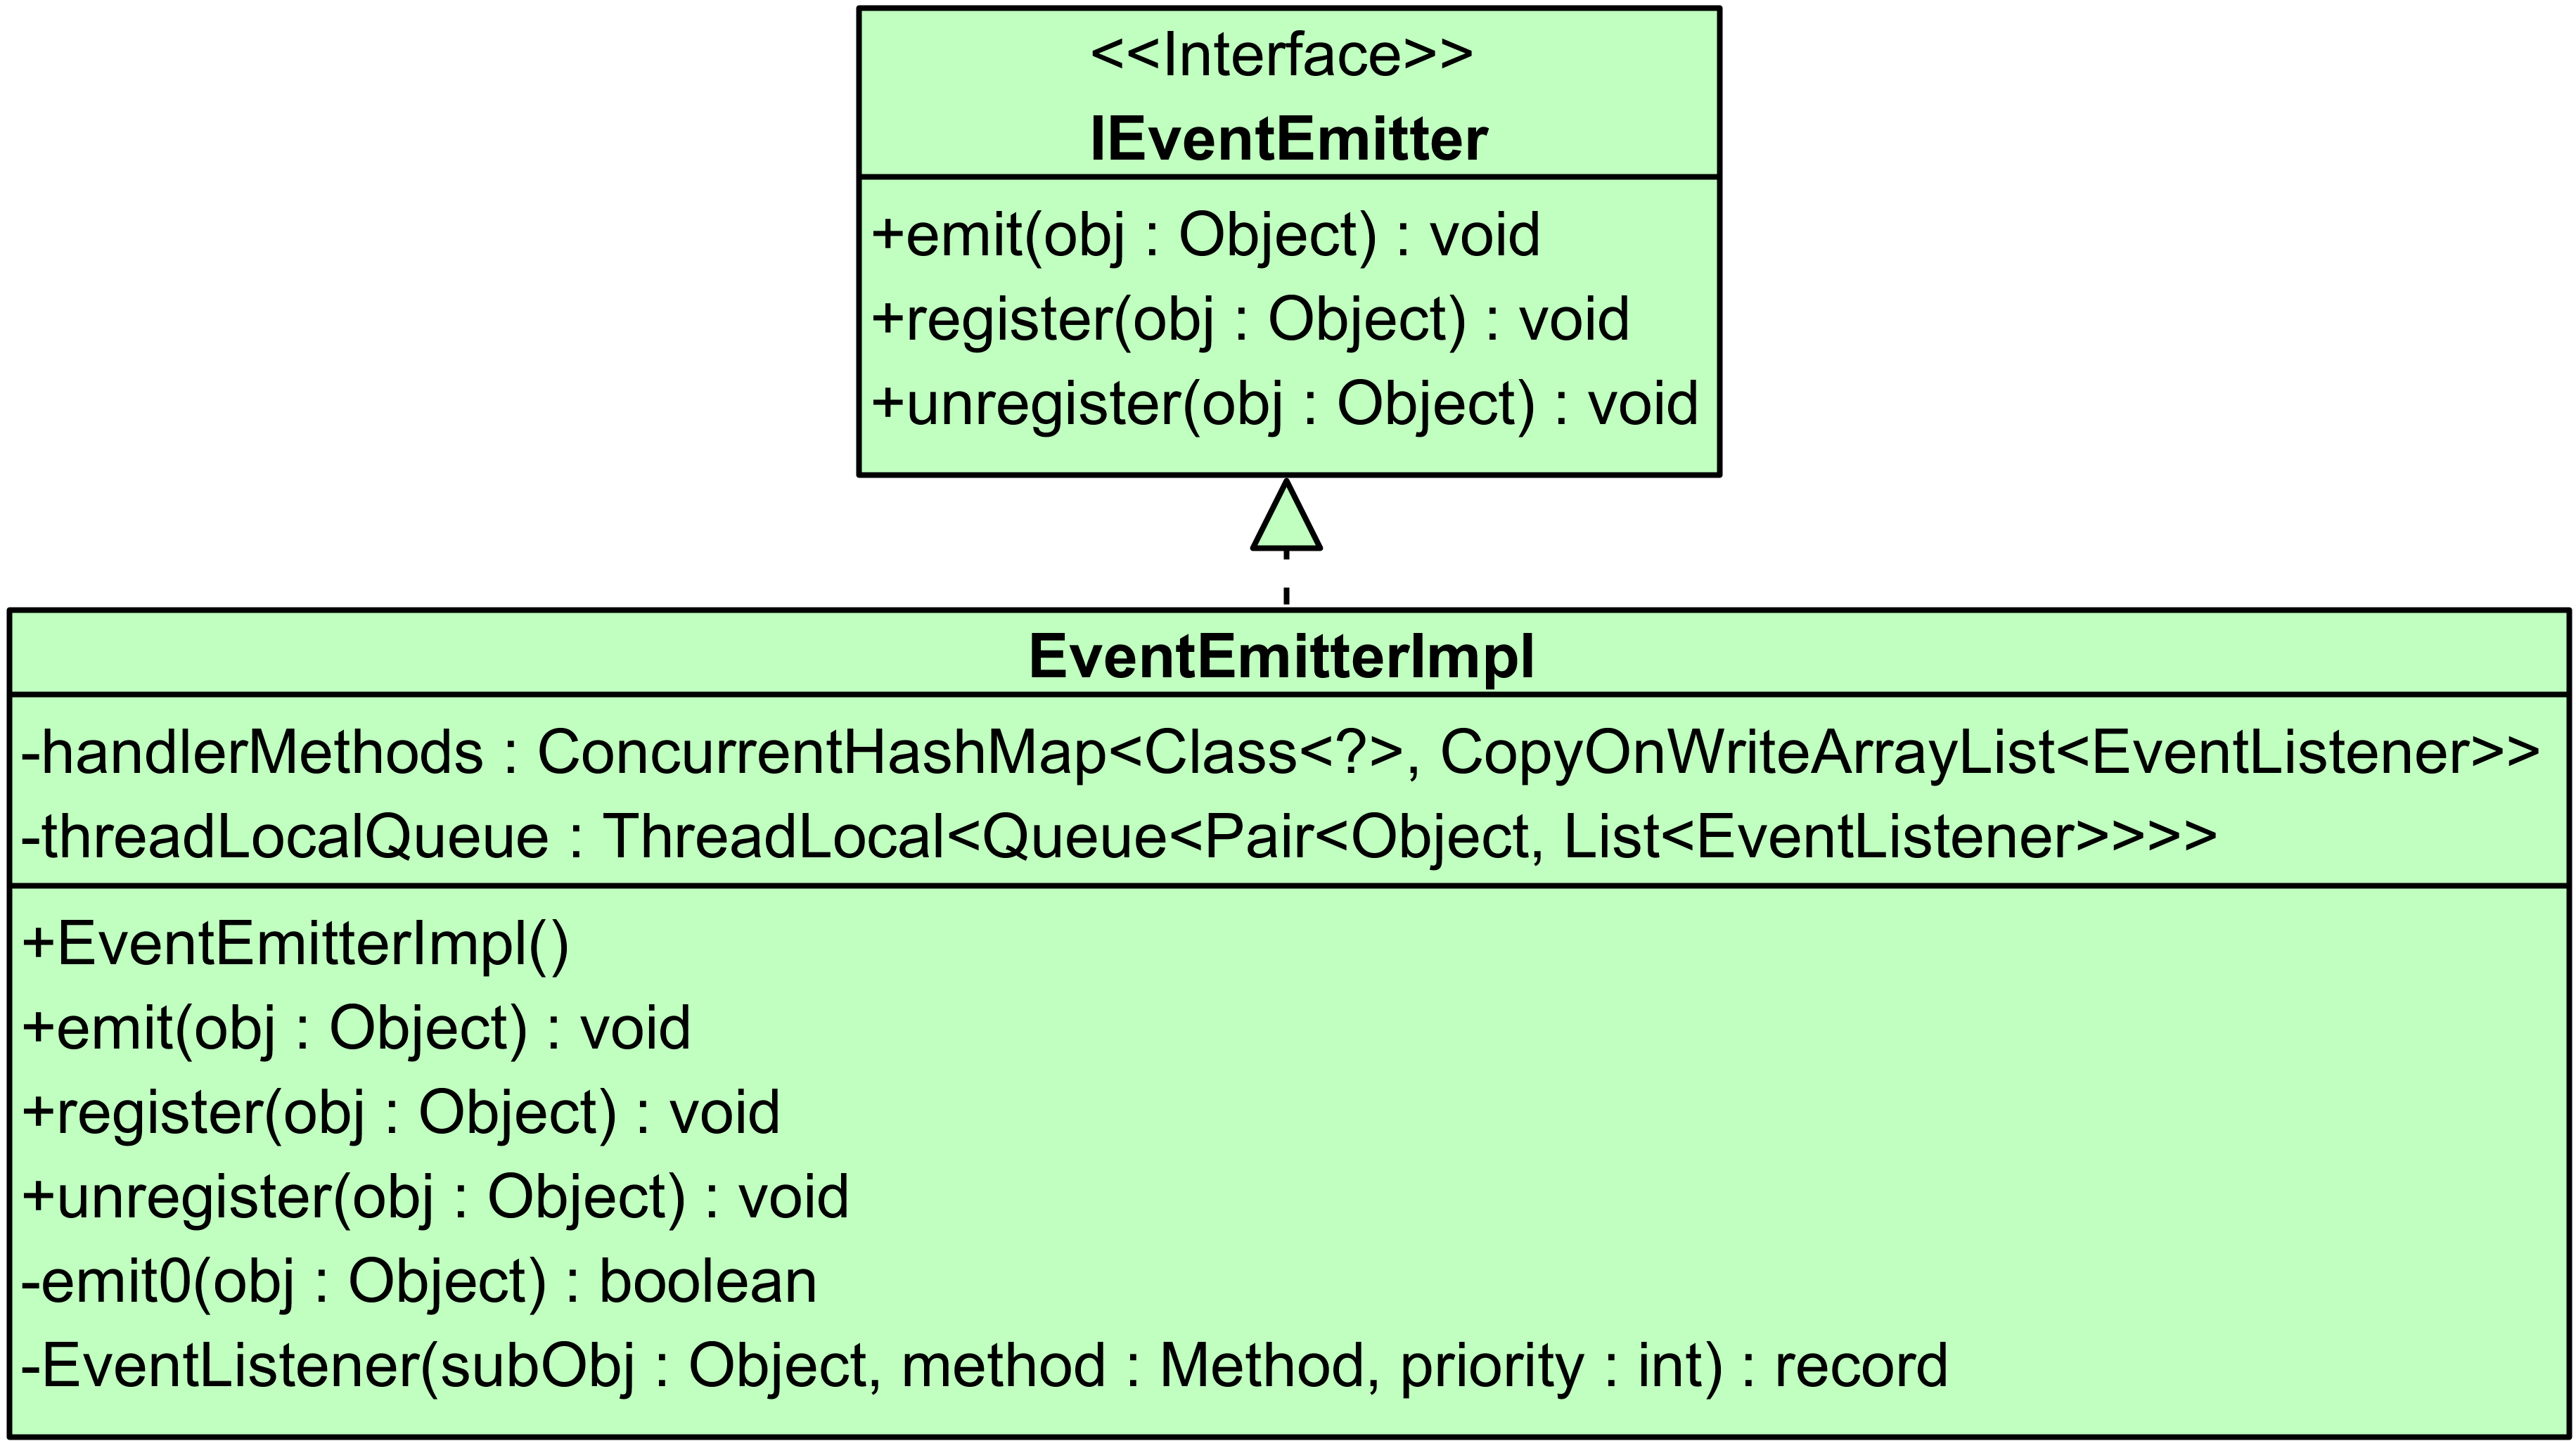
\includegraphics[width=\textwidth-4cm]{Abbildungen/EventEmitter.png}
	\caption{Diagramm -- IEventEmitter Schnittstelle und Implementierung}
	\label{fig:event_emitter}
\end{figure}
\noindent Mit der \texttt{IEventEmitter\#emit} Methode, wird dem System ein neues Event übermittelt und alle Methoden, welche für dieses Event registriert wurden, nach Priorität der Annotation aufgerufen. Die daraus resultierenden Methodenaufrufe werden dabei auf dem aufrufenden \texttt{Thread} ausgeführt und blockieren diesen, bis alle Aufrufe abgeschlossen wurden.
\subsection{Paket: events}
Das \texttt{events} Paket stellt eine Vielzahl an Standard-Events für beispielsweise den Lebenszyklus der Applikation (\texttt{InitEvent}, \texttt{StartEvent}, \texttt{StopEvent}) oder für Statusaktualisierungen des Preloaders (\texttt{StateChangeEvent}, \texttt{ProgressEvent}) bereit. Diese können durch eine \texttt{IEventEmitter} genutzt werden.
\subsection{Paket: application}
Die von \texttt{SimpliFX} verwalteten JavaFX Applikation- und Preloader-Klassen sowie die dafür benötigten Annotation sind im \texttt{application} Paket enthalten und definieren alle Methoden, welche durch die Applikation- respektive Preloaderklasse vererbt werden (siehe \autoref{fig:app_package}). Dabei wird bei der Erstellung der Klassen, eine für den Typ des Einstiegspunktes spezifische \texttt{IEventEmitter} Instanz übergeben, welche etwaige interne Methodenaufrufe in Form von vordefinierten Events an den vom Entwickler definierten, Einstiegspunkt delegiert.
\begin{figure}[H]
	\centering
	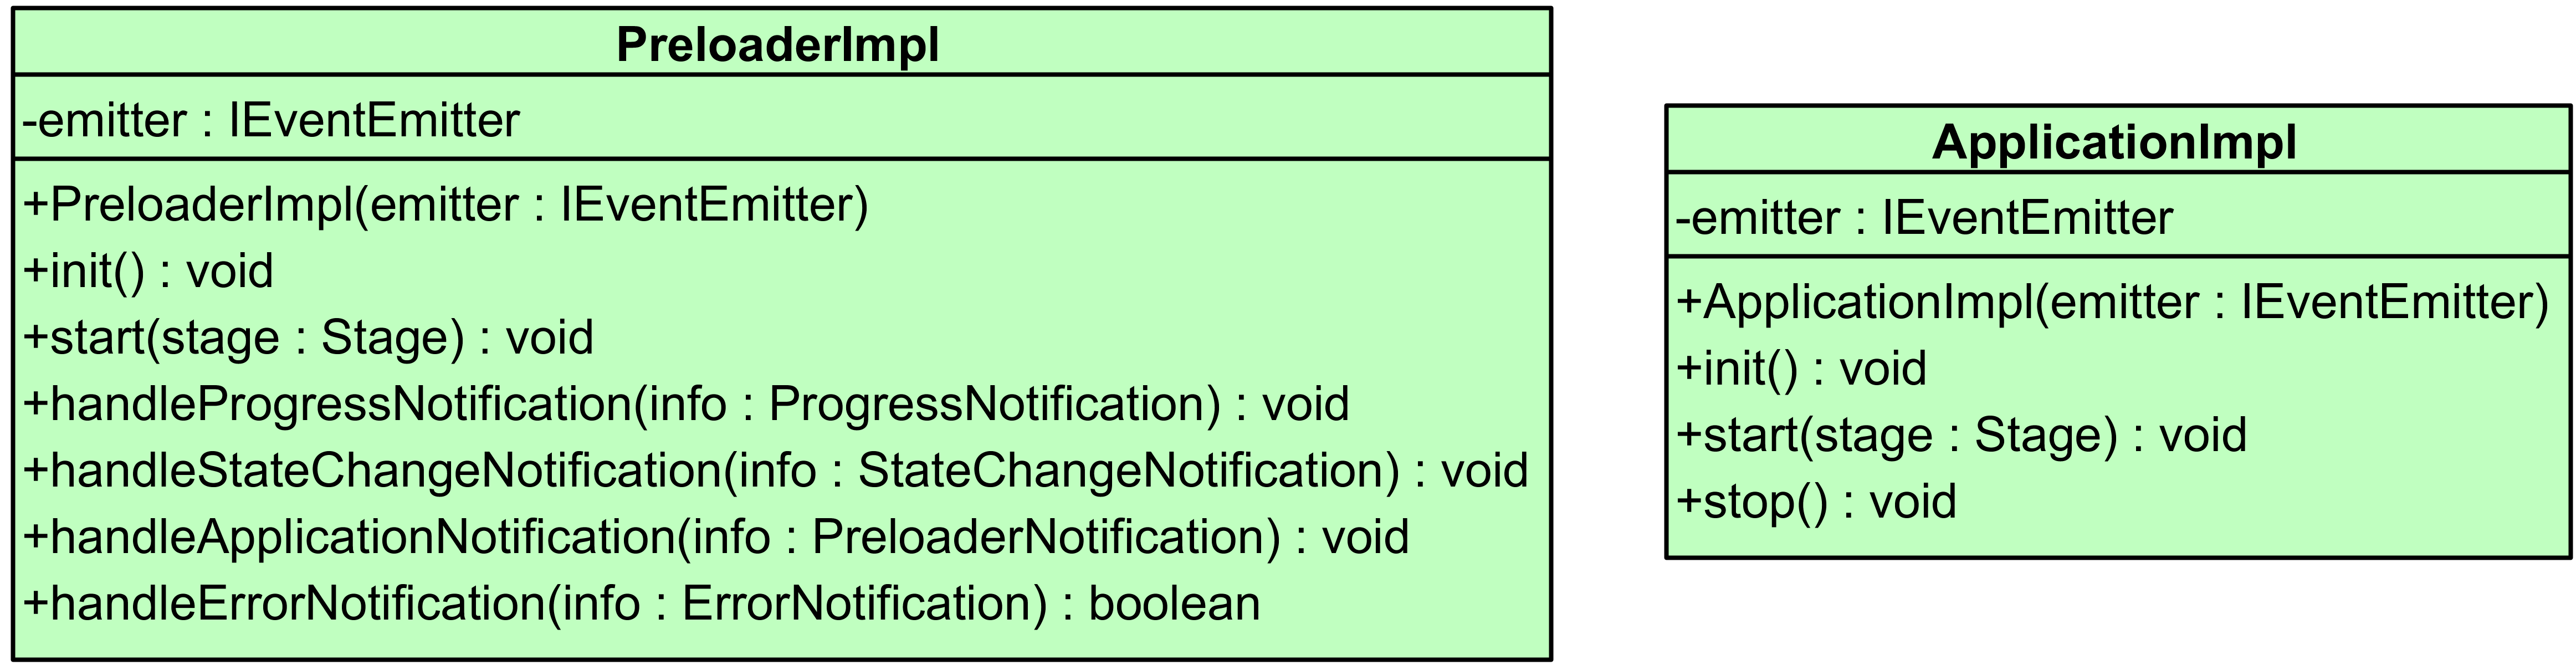
\includegraphics[width=\textwidth-2cm]{Abbildungen/Applikation und Preloader.png}
	\caption{Diagramm -- Applikation und Preloader.}
	\label{fig:app_package}
\end{figure}
\subsection{Paket: config}
Klassen für das Verwalten von Konfigurationsdateien und deren Injektion in Controllern sind im \texttt{config} Paket aufzufinden. Dabei werden ausschließlich Dateiformate unterstützt, welche mit der Java Properties API kompatibel sind.
\section{Essentielle Quelltextausschnitte}
In den folgenden Unterkapiteln werden wichtige Quelltextausschnitte, welche für Basisfunktionen von \texttt{SimpliFX} verantwortlich sind, dargestellt und näher erklärt.
\subsection{SimpliFXMLLoader}
\label{simplifxmlloader}
Der \texttt{SimpliFXMLLoader} unterstützt dieselbe XML-Syntax wie der \texttt{FXMLLoader}. Der einzige Unterschied liegt in der Verwendung von Übersetzungsschlüsseln aus Übersetzungsdateien. Das eigentliche Präfix zur Übersetzung (\glqq\texttt{\%}\grqq) wird automatisch durch den Loader in ein dynamisches Binding konvertiert. Ist die ursprüngliche Funktionalität der Übersetzung für bestimmte Elemente in der FXML Datei gewünscht, so kann das Präfix mit dem Voranstellen eines \glqq\texttt{!}\grqq{} erweitert werden. Der \texttt{SimpliFXMLLoader} unterstützt keine direkte Angabe von \texttt{ResourceBundle} Instanzen in den \texttt{load} Methoden oder den Konstruktoren. Stattdessen kann eine \texttt{II18N} Instanz übergeben werden. Um eine dynamische Übersetzung zu ermöglichen, musste das Behandeln von gefundenen Übersetzungsschlüsseln teilweise neu implementiert werden. Dazu wurde unter anderem die interne Methode \texttt{Element\#resolvePrefixedValue} (Zeilen 430--437) abgeändert. Ein einfaches Nutzen der \texttt{ResourceBundle\#getString} Methode ist für die gewünschte Dynamik ausgeschlossen. Stattdessen wurde eine neue innere Klasse definiert, welche das jeweils erstellte \texttt{StringBinding}, sowie den eigentlichen Übersetzungsschlüssel kapselt und Methoden zur Generierung von parametrisierten Schlüsseln zur Verfügung stellt (\autoref{fig:translatable_property}). Die neue Implementierung der Ressourcenbehandlung ist in \autoref{lst:resource_handling} dargestellt.
\begin{figure}[H]
	\centering
	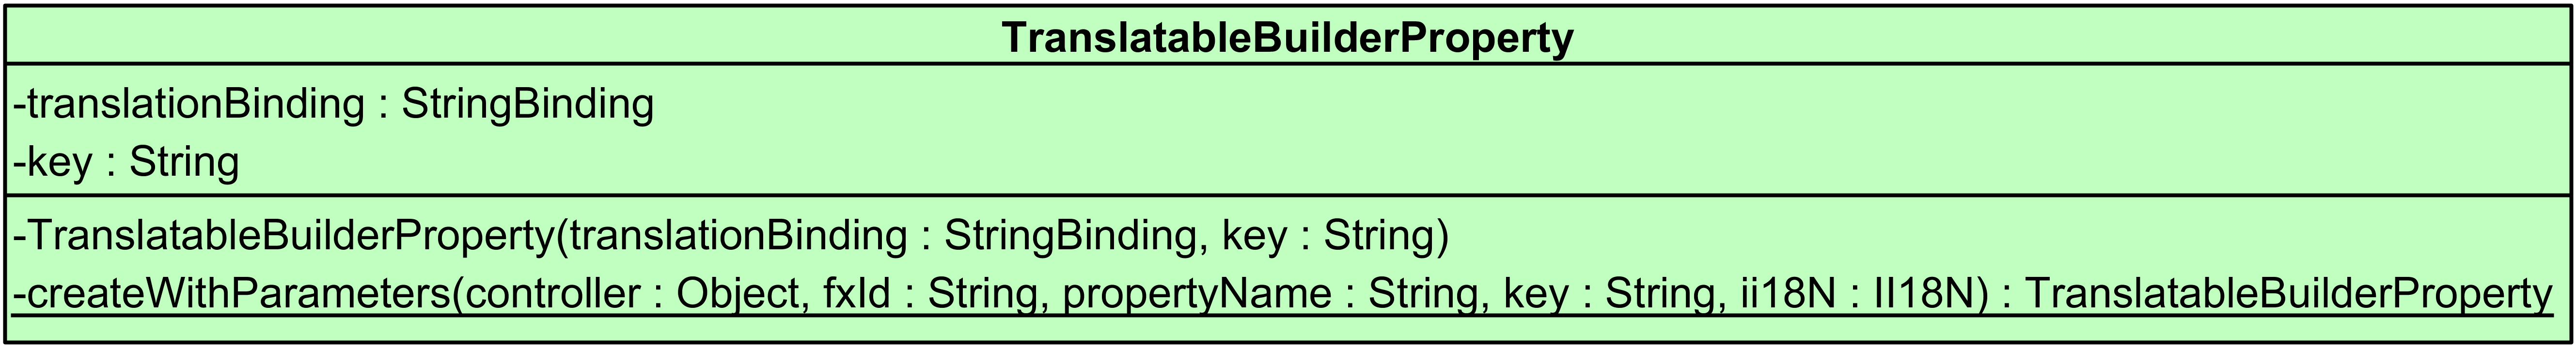
\includegraphics[width=\textwidth]{Abbildungen/Ressourcenbehandlung.png}
	\caption{Diagramm -- Klasse zur Datenkapselung von Übersetzungsinformationen}
	\label{fig:translatable_property}
\end{figure}
\noindent Der Zugriff auf interne Properties von einfachen JavaFX-Komponenten wie zum Beispiel \texttt{Button} oder \texttt{Label} wird durch einen \texttt{BeanAdapter} ermöglicht, welcher automatisch durch den \texttt{FXMLLoader} erstellt wird. Mit diesem Adapter können Property-Felder auch nach Instanziierung der eigentlichen Komponentenklasse modifiziert und ausgelesen werden. Komplexe Komponenten wie \texttt{AreaChart}, werden mithilfe von \texttt{ProxyBuilder} Instanzen erstellt. Daraus resultiert, dass zum Zeitpunkt der Ressourcenbehandlung noch kein Objekt der Klasse instanziiert worden ist und trivialerweise kein Zugriff auf die internen Properties möglich ist. Aus dem Grunde wird am Anfang der Behandlung überprüft, ob ein \texttt{BeanAdapter} für die aktuelle JavaFX-Komponente erstellt worden ist und anhand dessen das weitere Vorgehen bestimmt. Ist ein solcher Adapter präsent, kann ein \texttt{StringBinding} für die aktuelle Property aus der FXML Datei erstellt und bei vorhandenem Controller direkt mit eventuellen Parametern verknüpft werden. Andernfalls ist eine Erstellung eines \texttt{StringBinding}s für den Schlüssel an dieser Stelle nicht möglich. Für letztere Fälle wurden vereinzelte andere Quelltextabschnitte des Loaders modifiziert, auf welche hier aber nicht näher eingegangen wird.
\begin{figure}[H]
	\centering
	\begin{lstlisting}[caption=Implementierung -- Ressourcenbehandlung im \texttt{SimpliFXMLLoader}, captionpos=b, label=lst:resource_handling]
if (valueAdapter != null) {
	ObservableValue<?> val = valueAdapter.getPropertyModel("id");
	if (val instanceof StringProperty property && controller != null 
			&& propertyName != null) {
		return TranslatableBuilderProperty
				.createWithParameters(controller, property.get(), 
						propertyName, aValue, ii18N);
	}
	return new TranslatableBuilderProperty(ii18N
			.createBindingForKey(aValue), aValue);
} else {
	return new TranslatableBuilderProperty(null, aValue);
}
	\end{lstlisting}
\end{figure}
\subsection{Erweiterbare Abhängigkeitsinjektion}
Im Rahmen der Erweiterbarkeit (\autoref{nreq26}) wurde das System zur Abhängigkeitsinjektion weitgehend abstrakt gehalten. Wie in \autoref{package_di} erläutert und in \autoref{appendix:add_new_di_library} beispielhaft implementiert, ist es möglich neue Bibliotheken zur Laufzeitinjizierung hinzuzufügen, ohne dass \texttt{SimpliFX} Komponenten abgeändert werden müssen. Dazu werden alle Annotationen des Einstiegspunktes auf die Meta-Annotation \texttt{@DIAnnotation} überprüft. Ein exemplarischer Quelltextausschnitt, welcher dieses Konzept implementiert, ist in \autoref{lst:reflective_di} zu erkennen. Eine ähnliche Implementierung ist in \texttt{SimpliFX} verwendet worden.
\begin{figure}[H]
	\centering
	\begin{lstlisting}[caption=Implementierung -- Abhängigkeitsinjektion, captionpos=b, label=lst:reflective_di, basicstyle={\scriptsize\ttfamily}]
// Besitzt die Annotation die Meta-Annotation @DIAnnotation?
if (annotation.annotationType().isAnnotationPresent(DIAnnotation.class)) {
	// Finde IDIEnvironmentFactory Implementierung durch Annotationsparameter
	var factory = annotation.annotationType().getAnnotation(DIAnnotation.class)
			.value();
	// Starte Reflection-Prozess mit Factory als Einstiegspunkt
	ClassReflection classRef = Reflection.reflect(factory);
	// Finde Standardkonstruktor
	Optional<ConstructorReflection> constructorRefOpt = classRef.hasConstructor();
	if (constructorRefOpt.isEmpty()) {
		// Fehler - Kein Standardkonstruktor gefunden
		break;
	}
	// Erstelle neue Instanz der Factory
	IDIEnvironmentFactory<?> factoryInstance = constructorRefOpt.get()
			.instantiateUnsafeAndGet();
	// Finde einzige Methode der Factory
	MethodReflection methodRef = Reflection.reflect(factoryInstance)
			.reflectMethod("create", Object.class, 
					(Class<?>) ((ParameterizedType) factory.getGenericInterfaces()[0])
					.getActualTypeArguments()[0]);
	// Erstelle eine neue DIEnvironment Instanz
	DIEnvironment env = methodRef.invokeUnsafe(applicationListener, annotation);
	break;
}
	\end{lstlisting}
\end{figure}
\chapter{Evaluation}
\label{evaluation}
Im folgenden Kapitel werden Kernkonzepte von \texttt{SimpliFX} durch Quelltextbeispiele und eine Beispielanwendung erklärt. Außerdem wird eine Applikation erstellt, welche äquivalente Funktionalitäten wie die Beispielanwendung aufweist, aber vollständig auf die Nutzung von \texttt{SimpliFX} verzichtet. Beide Anwendungen werden in verschiedenen Aspekten wie der Benutzerfreundlichkeit oder dem Zeitaufwand verglichen und die Ergebnisse werden abschließend in einem Fazit zusammengefasst. 
\add{Intro}

\section{Entwicklung von Beispielsoftware}
\label{entwicklung_von_beispielsoftware}
%\subsection{Voraussetzungen}
\add{maybe add comment}
\noindent Bevor die Entwicklung der eigentlichen Software begonnen werden kann, müssen etwaige externe Bibliotheken wie JavaFX für \texttt{SimpliFX} bereitgestellt werden. Außerdem muss \texttt{SimpliFX} zur Kompilierzeit im Klassenpfad der zu entwickelnden Anwendung existieren. Da die Bibliothek im Github Maven-Repository verfügbar ist, wird der folgende Entwicklungsprozess sowie die Verwaltung von externen Bibliotheken durch die Verwendung von Maven unterstützt. In der \texttt{pom.xml} müssen für eine volle Funktionalität folgende Artefakte als Abhängigkeiten deklariert werden:
\begin{itemize}
	\item \texttt{de.intelligence:simplifx-guice} für das Nutzen aller Basisfunktionen von \texttt{SimpliFX} und der Kompatibilität zu Guice für die Abhängigkeitsinjektion.
	\item \texttt{org.openjfx:javafx-controls:16} für Kontrollkomponenten wie z.B. Schaltflächen.
	\item \texttt{org.openjfx:javafx-fxml:16} für das Verwenden von FXML Dateien.
	\item \texttt{org.openjfx:javafx-graphics:16} für das Darstellen von Komponenten im Szenengraph. Außerdem muss bei der Artefaktdeklaration die jeweilige Zielplattform als \texttt{classifier} angegeben werden. Ein Beispiel für die Windows-Plattform ist nachfolgend dargestellt.
	\begin{lstlisting}[language=XML, frame=none, belowskip=0pt]
<dependency>
    <groupId>org.openjfx</groupId>
    <artifactId>javafx-graphics</artifactId>
    <version>16</version>
    <classifier>win</classifier>
</dependency>	
	\end{lstlisting}
	\item \texttt{com.jfoenix:jfoenix:9.0.10} für erweiterte Designkomponenten.\footnote{Die neuste Version von JFoenix ist aufgrund der Jigsaw-API nicht direkt mit Java 16 kompatibel. Um die Bibliothek dennoch zu verwenden, werden eventuelle, auf das Modularitätssystem zurückführbare, Probleme durch das Nutzen der Reflection-Schnittstelle gelöst.}
\end{itemize}
Die vollständige \texttt{pom.xml} sowie alle in diesem Unterkapitel erstellten Klassen und Dateien sind im öffentlichen Github Maven-Repository unter dem Artefakt \texttt{de.intelligence:demo-applications} einsehbar.
\subsection{Struktur und Funktion der Beispielanwendung}
Die Anwendung soll weitgehend alle Funktionen von \texttt{SimpliFX} in Anspruch nehmen. Um die Konfigurationsschnittstelle sowie die Abhängigkeitsinjektion demonstrativ zu zeigen, wird eine Konfigurationsdatei definiert, welche Zugangsdaten und Verbindungsparameter zu einem imaginären Server enthält. Dazu wird ein Service erstellt, welcher für die Behandlung des Loginprozesses verantwortlich ist und durch ein Guice Modul zur Verfügung gestellt wird. Für die dynamische Lokalisierungsfunktion wird ein \texttt{ResourceBundle} mit dem Basisnamen \texttt{Messages} in sowohl der deutschen als auch der englischen Sprache erstellt. Wenn die Anwendung gestartet wird, soll eine grafische Schnittstelle für ein exemplarisches Einloggen angezeigt werden, welche Standardfunktionen wie das Eingeben der Zugangsdaten sowie die Änderung der Standardsprache zulassen soll. Die Funktion zur Sprachänderung kann dabei durch eine JavaFX \texttt{MenuBar} erfolgen. Wenn ein eventueller Login erfolgreich war, soll dem Entwickler eine Seitenleiste sowie ein Bereich, dessen Inhalt durch ebendiese kontrolliert wird, präsentiert werden. Die Seitenleiste soll vier Schaltflächen zur Navigation durch die Testapplikation, sowie ein Textfeld, welches die Verbindungsdaten zum Server anzeigt, enthalten. Der Startcontroller wird im folgenden als \texttt{MainController} bezeichnet. 
Dieser Controller hat als Wurzelelement eine \texttt{BorderPane} und erstellt zwei Controller Untergruppen in dieser. Im oberen Bereich wird die \texttt{titleBar} Gruppe initialisiert, welche Anwendungseinstellungen unabhängig vom aktuell angezeigten Controller bereitstellt und im Mittelbereich die \texttt{mainContent} Gruppe, welche die Darstellung der eigentlichen Anwendung übernimmt und beim Start den \texttt{LoginController} als aktiven Controller anzeigt. Die \texttt{mainContent} Gruppe beinhaltet außerdem den \texttt{MainMenuController}, welche wiederum eine linke Seitenleiste sowie einen Bereich für andere Inhalte neben dieser verwaltet. Eine Übersicht aller verwendeten Controller und Controllergruppen ist in \autoref{fig:controller_relations} abgebildet. Blaue Kreise sind dabei Gruppen, rot hervorgehobene Controller stellen den Startcontroller in der jeweiligen Gruppe dar und Linien, welche einen oder mehrere Controller verbinden, spezifizieren das Subcontroller Verhalten. Wenn beispielsweise der \texttt{MainMenuController} der aktive Controller in der \texttt{mainContent} Gruppe ist und zum \texttt{LoginController} gewechselt wird, so werden auch entsprechende Lebenszyklusmethoden im aktiven Controller von \texttt{sidebarContent} und \texttt{sidebar} aufgerufen.
\begin{figure}[H]
	\centering
	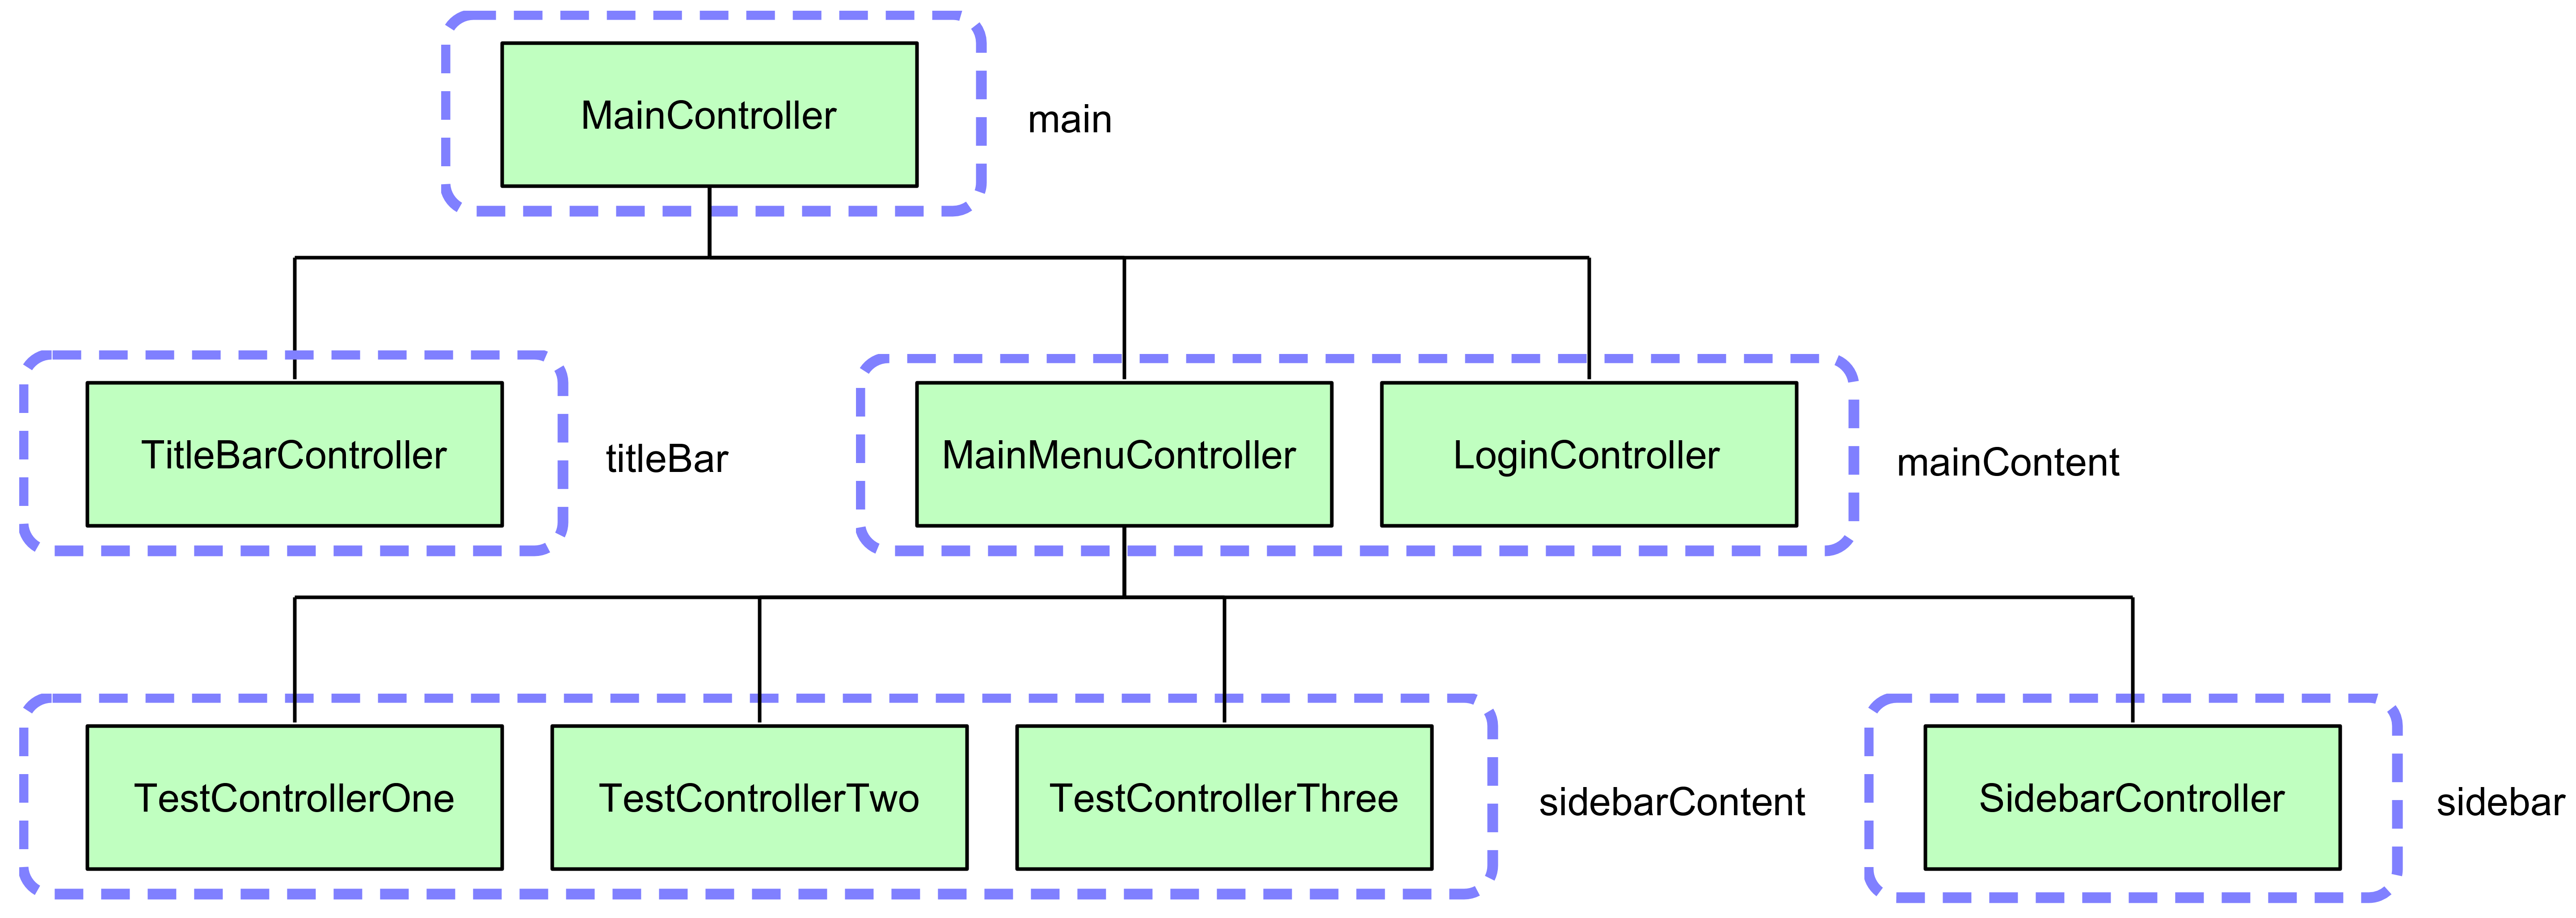
\includegraphics[width=\textwidth]{Abbildungen/Controller Relations.png}
	\caption{Diagramm -- Controller und Controllergruppen.}
	\label{fig:controller_relations}
\end{figure}
\subsection{Implementierung der Beispielanwendung}
Damit eine \texttt{SimpliFX} Anwendung als solche erkannt wird, muss eine Klasse definiert werden, welche als Einstiegspunkt dienen soll. Diese muss die Annotation \texttt{@ApplicationEntryPoint} aufweisen und als Parameter den Startcontroller (\texttt{MainController}) übergeben. Für die Abhängigkeitsinjektion mit Guice muss der Einstiegspunkt auch mit \texttt{@GuiceInjection} annotiert werden und die Klasse eines Guice-Moduls übergeben. Wie in der Einleitung bereits beschrieben, wird das Modul nur die Implementierung des Login Services bereitstellen (siehe \autoref{fig:login_service}). 
\begin{figure}[H]
	\centering
	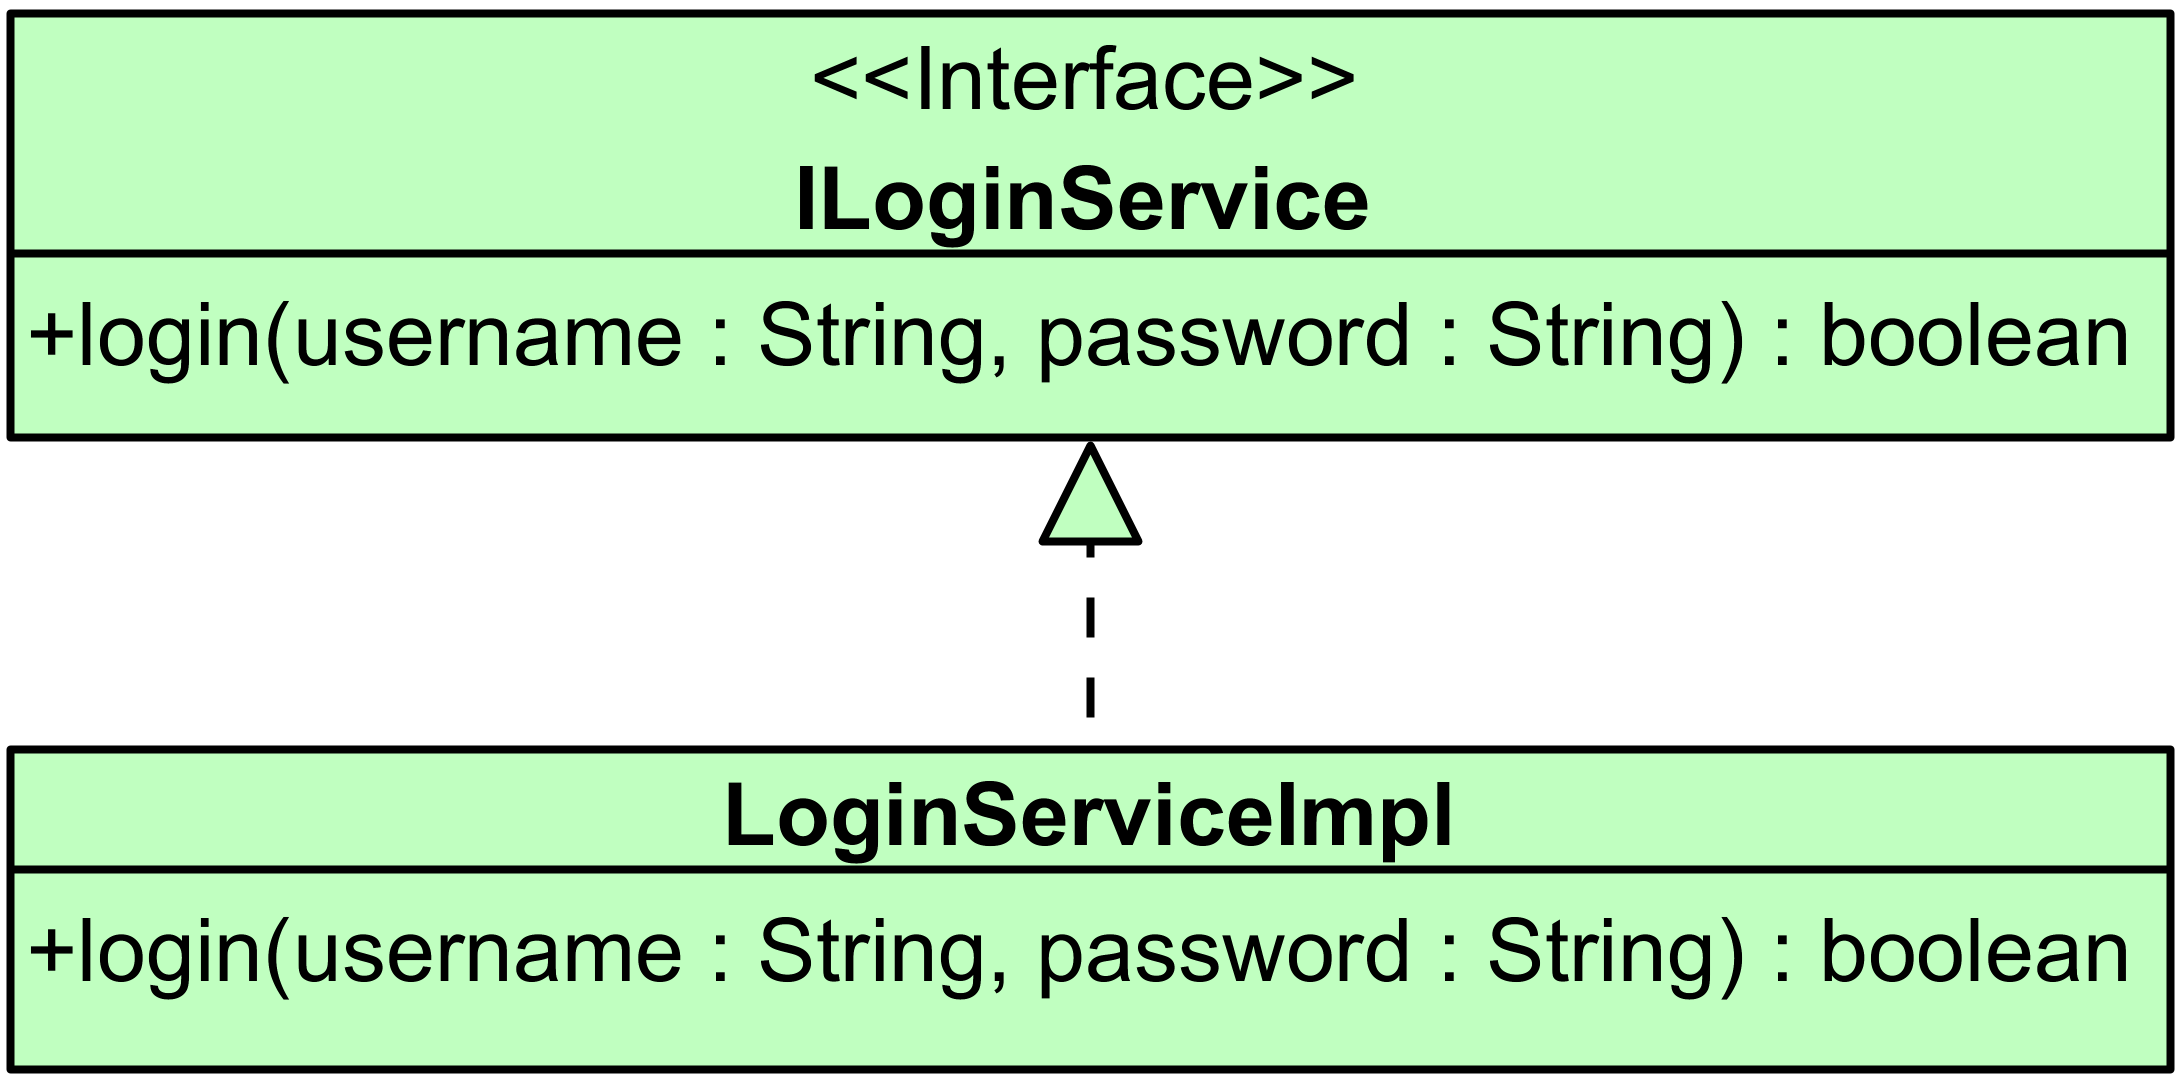
\includegraphics[width=\textwidth]{Abbildungen/Login Service.png}
	\caption{Diagramm -- Login Service.}
	\label{fig:login_service}
\end{figure}
\noindent Dazu werden noch Konfigurationsänderungen der \texttt{Stage} in Form von Symbol und Titeländerungen durchgeführt. Eine minimale Version des Einstiegspunktes ist in \autoref{lst:entry_point_demo} zu sehen. Dabei wird in Zeile Eins der Titel der \texttt{Stage} auf \texttt{Login} gesetzt und ein Symbol für die Fensterleiste angegeben. Danach wird der Hauptcontroller in der zweiten Zeile definiert, indem die jeweilige Controllerklasse als Parameter übergeben wird. Abschließend wird die Guice Kompatibilität aktiviert und ein Modul festgelegt (Zeile Drei).
\begin{figure}[H]
	\begin{lstlisting}[caption=Demo -- Minimaler Einstiegspunkt., captionpos=b, label=lst:entry_point_demo, numbers=left, xleftmargin=1.5em, framexleftmargin=1.5em]
#@StageConfig(title = "Login", icons = "icon.png")
#@ApplicationEntryPoint(MainController.class)
#@GuiceInjection(MainModule.class)
public final class DemoApplication {}
	\end{lstlisting}
\end{figure}
\noindent Für das Nutzen der dynamischen Übersetzung und der Konfigurationsschnittstelle müssen dem Einstiegspunkt zwei Felder hinzugefügt werden (\autoref{lst:fields_demo}). Außerdem sollen Subcontroller die Möglichkeit haben, den Titel der \texttt{Stage} abzuändern, weshalb die \texttt{titleProperty} als geteilte Ressource definiert wird und beim Start der Anwendung in einer \texttt{EventHandler} Methode gesetzt wird (\autoref{lst:event_method_demo}).
\begin{figure}[H]
	\begin{lstlisting}[caption=Demo -- Benötigte Felder., captionpos=b, label=lst:fields_demo]
#@ResourceBundle((@\tikzmark{resLeft}{}@)"lang.Messages"(@\tikzmark{resRight}{}@))
private II18N ii18N;

#@ConfigSource((@\tikzmark{conLeft}{}@)"config/connection"(@\tikzmark{conRight}{}@))
private Properties properties;

#@Shared
private SharedReference<StringProperty> (@\tikzmark{titleLeft}{}@)titleRef(@\tikzmark{titleRight}{}@);(@\begin{tikzpicture}[overlay,remember picture]
	\node[draw](resources) at (-0.5,3) {Pfad zum ResourceBundle};
	\node[draw](config) at (0.4,2) {Pfad zur Konfigurationsdatei};
	\node[draw](title) at (0.4,1) {Geteilte Ressource für Titel};
	\foreach \x/\y in {con/red,title/blue} {
		\DrawOverBar[-,\y,thick]{\x Left.north}{\x Right.north}
	}
	\DrawArrow[blue, in=280, out=-280]{title}{title}{0,-0.2}
	\DrawArrow[red, in=150, out=10]{con}{config}{-3.05,0.0}
	\renewcommand{\VerticalShiftForBar}{0em, -1.6ex}
	\renewcommand{\Stub}{0em, 0.3em}
	\DrawOverBar[-, green, thick]{resLeft.north}{resRight.north}
	\renewcommand{\VerticalShiftForArrows}{0, -1ex}
	\DrawArrow[green, in=215, out=-10]{res}{resources}{-2.3,-0.25}

\end{tikzpicture}@)
	\end{lstlisting}
\end{figure}
\begin{figure}[H]
	\begin{lstlisting}[caption=Demo -- Start EventHandler., captionpos=b, label=lst:event_method_demo]
#@EventHandler
private void onStart(StartEvent event) {
	// Titel Property setzen
    this.titleRef.set(event.getStage().titleProperty());
	// Stage zeigen
    event.getStage().show();
}
	\end{lstlisting}
\end{figure}
\noindent Zum Starten der Anwendung muss der Hauptcontroller korrekt deklariert werden und eine \texttt{main} Methode existieren, welche \texttt{SimpliFX\#launch} aufruft. Außerdem muss, aufgrund der Inkompatibilität zwischen JFoenix und Java 16, per Reflection-Schnittstelle eine \texttt{add-opens} Direktive vor der eigentlichen Initialisierung von \texttt{SimpliFX} und \texttt{JavaFX} hinzugefügt werden.\footnote{JFoenix Issue: \url{https://github.com/sshahine/JFoenix/issues/1052}} Der Einfachheit halber wird die \texttt{main} Methode in der \texttt{DemoApplication} Klasse deklariert (\autoref{lst:main_method_demo}).
\begin{figure}[H]
\begin{lstlisting}[caption=Demo -- \texttt{main} Methode., captionpos=b, label=lst:main_method_demo]
public static void main(String[] args) throws Exception {
    Reflection.addOpens("java.lang.reflect", "java.base",
			JFXTextFieldSkin.class.getModule());
    SimpliFX.launch();
}
	\end{lstlisting}
\end{figure}
\noindent Der funktionsfähige Einstiegspunkt der Anwendung ist noch einmal vollständig in \autoref{lst:entry_point_demo_full} dargestellt.\\
Wird zu diesem Zeitpunkt versucht, die Applikation zu starten, so wird diese mit einem Fehler terminieren, da der angegebene Hauptcontroller noch nicht erstellt und konfiguriert wurde.
\add{TODO CONTINUE}
\noindent...\\
...\\
...\\
\notebox{Die Höhe und die Breite einer Controllergruppe richtet sich immer nach dem aktuell angezeigten Controller. \texttt{SimpliFX} nutzt dazu das \texttt{prefHeight}- und \texttt{prefWidth} Attribut des jeweiligen Wurzelelementes. Ist kein solches Attribut gesetzt worden, werden Standardwerte genutzt.}
\section{Vergleich konventioneller Methoden mit entwickeltem System}
\label{vergleich_system_javafx}

\add{Vergleich konventioneller Methoden mit entwickeltem System}

\chapter{Fazit}
\label{fazit}
In dieser Arbeit wurde eine auf Java Annotationen basierende Bibliothek zur Simplifizierung und Expansion von JavaFX konzipiert und implementiert. Vorhandene Funktionen wurden in einer Problemanalyse auf Komplexität und Vollständigkeit untersucht und die daraus resultierenden Probleme dienten als Grundlage für die Anforderungsanalyse. Die identifizierten funktionalen und nicht-funktionalen Anforderungen wurden für die Entwicklung eines Konzeptes genutzt, welches wiederum das Fundament der vollständigen Systemimplementierung bildete und dabei wurde ein besonderer Fokus auf die explizite Erfüllung aller Ziele gesetzt. In der prototypischen Implementierung wurden alle erforderlichen Anforderungen mit spezieller Berücksichtigung von paradigmatischen softwaretechnischen Qualitätsrichtlinien wie der Erweiterbarkeit und der Wartbarkeit eines Systems erfüllt. Abschließend wurde der Funktionsumfang von JavaFX mit dem von \texttt{SimpliFX} im Rahmen der Evaluation verglichen. 

\section{Zusammenfassung und Bewertung}
\label{zusammenfassung}
Gemäß der in der Einleitung beschriebenen Zielsetzung wurde eine Bibliothek entwickelt, welche das Arbeiten und die Entwicklung von Applikationen mit JavaFX in einigen Kernkonzepten vereinfacht (siehe \autoref{zielsetzung}). Besonders die Sprachunterstützung und die dafür benötigte dynamische Übersetzung durch einen neuen \texttt{FXMLLoader} sowie eine Erweiterung der Funktionen für eine Erstellung und Verwaltung von Controllern, sind ein fundamentaler Bestandteil der Bibliothek. Des Weiteren können Konfigurationsdateien und Sprachdateien mit Leichtigkeit durch Annotationsverwendung geladen und nach Initialisierung der Anwendung genutzt werden. Außerdem wurden Schnittstellen hinzugefügt, welche die Interaktion zu komplexen Systemen wie der Java Reflection API vereinfachen und effektiv die Fehleranfälligkeit dieser durch eine zentralisierte Fehlerbehandlung reduzieren. Insgesamt wurden im Rahmen der Anforderungsanalyse (siehe \autoref{anforderungsanalyse}) \thereq{} Anforderungen an die Bibliothek gestellt. Diese setzen sich aus \thereqFunAmount{} fundamentalen und \NUMBERFORMAT{\thereqOptAmount{}} optionalen Anforderungen zusammen, von welchen jeweils \thereqFunCompleted{} bzw. \NUMBERFORMAT{\thereqOptCompleted{}} erfüllt worden sind. Daraus resultiert eine Erfüllquote von \CalculatePercentage{\thereqFunCompleted}{\thereqFunAmount} der fundamentalen Anforderungen und eine von \CalculatePercentage{\thereqOptCompleted}{\thereqOptAmount} bei den optionalen Anforderungen. Zusammenfassend wurden demnach \CalculatePercentage{\thereqTotalCompleted}{\thereq} aller Anforderungen erfüllt. Wenn eine Anforderung nicht erfüllt wurde, lag dies am Umfang, welcher dann mit einem hohen Zeitaufwand einhergehen würde. In \autoref{tab:requirements} ist eine Gesamtübersicht dieser Anforderungen mit den jeweiligen Erfüllungsstatus zu finden. Auch wenn es sich bei der entwickelten Bibliothek keinesfalls um ein vollkommen abgeschlossenes Projekt handelt und bei der aktiven Entwicklung von Testfällen und der generellen Erhöhung der Testabdeckung mit hoher Wahrscheinlichkeit noch Fehler im Quelltext detektiert werden, kann diese dennoch für andere Projekte verwendet werden und Neueinsteigern in die Java- bzw. JavaFX-Welt als Hilfestellung dienen.

\newcounter{index}

\NewDocumentCommand{\myfunc}{ >{\SplitList{,}} m }{\ProcessList{#1}{\func}}

\NewDocumentCommand{\func}{m}{\stepcounter{index}\ifnum\value{index}=6\setcounter{index}{1}\fi\ifnum\value{index}=5\IfNoValueTF{#1}{\xmark}{\cmark}\ifthenelse{\thetextCounter < \thereq}{\\\hline}{}\else\ifthenelse{\equal{\value{index}}{4}}{\IfNoValueTF{#1}{\xmark}{\cmark}&}{\ifthenelse{\equal{\value{index}}{2}}{\ifthenelse{\equal{#1}{freq}}{F}{NF}&}{#1&}}\fi}
\ExplSyntaxOn
\NewDocumentCommand{\myList}{sm}{\IfBooleanTF{#1}{\holene_mylist:o{#2}}{\holene_mylist:n{#2}}}
\newcounter{textCounter}
\seq_new:N \l_holene_mylist_input_seq%
\cs_new_protected:Npn \holene_mylist:n #1 {\seq_set_split:Nnn \l_holene_mylist_input_seq {;} { #1 }\seq_map_inline:Nn \l_holene_mylist_input_seq{\stepcounter{textCounter}\myfunc{##1}}} %\myfunc{##1}
\cs_generate_variant:Nn \holene_mylist:n {o}%
\ExplSyntaxOff
\StrLen{\fullreqs}[\AllStrLen]
\newcounter{lenCtr}
\setcounter{lenCtr}{\AllStrLen}
\StrMid{\fullreqs}{0}{\the\numexpr\value{lenCtr}-1\relax}[\FullConverted]

\begin{table}[H]
	\small
	\centering
	\begin{tabular}{|wc{0.03\textwidth}|wc{0.05\textwidth}|p{0.65\textwidth}|wc{0.05\textwidth}|wc{0.058\textwidth}|}
		\hline
		Nr. & Typ & Anforderung & Opt. & Erfüllt\\
		\hline
		\myList*{\FullConverted}\\\hline
	\end{tabular}
	\caption{Anforderungsliste}
	\label{tab:requirements}
\end{table}

\section{Ausblick und mögliche Erweiterungen}
\label{ausblick_und_mögliche_erweiterungen}
Im Folgenden werden mögliche Erweiterungen der implementierten Bibliothek vorgestellt. Auch wenn ein Großteil der Anforderungen durch das System erfüllt wird, existieren zu diesem Zeitpunkt noch einige optionale Anforderungen, welche nur teilweise bis gar nicht implementiert worden sind. Dazu gehört beispielsweise eine Annotationsvalidierung zur Kompilierzeit einer auf \texttt{SimpliFX} basierenden Applikation (\autoref{freq22}), was zu einer Detektion von Syntaxfehlern oder eventueller Inkorrektheiten in Konfigurationen führt. Wird eine solche Fehlkonfiguration entdeckt, kann ein Kompilierfehler durch einen Annotationsprozessor ausgelöst und Laufzeitausnahmen somit effektiv vermieden werden.\\
Die Unterstützung von Konfigurationsdateien ist in den Aspekten des Dateiformats und der zugelassenen Operationen stark begrenzt. Neben dem Akzeptieren von Properties- und \ac{xml}-Dateien, könnten beispielsweise noch weitere bekannte Konfigurationsformate wie \ac{json} oder \ac{yaml} durch \texttt{SimpliFX} erkannt und genutzt werden. Auch ist es momentan nicht möglich, eine schreibende Operation auf Konfigurationsdateien vorzunehmen, da zwischen Ressourcen im Klassenpfad und externen Ressourcen differenziert werden müsste und es generell kompliziert ist, Dateien zu modifizieren, welche sich innerhalb eines Java Archivs befinden.\\
Das System könnte ebenfalls um vom Betriebssystem des Nutzers abhängige Funktionen erweitert werden. Das Fensterdesign für eine JavaFX \texttt{Stage} kann durch die Nutzung des \ac{jni} ergänzt werden. Unter Windows kann somit beispielsweise ein Unschärfeeffekt des Fensterhintergrundes realisiert oder eine Modifikation der Titelleiste ermöglicht werden. Auch könnte eine Schnittstelle entwickelt werden, welche eine direkte Interaktion mit der Taskleiste ermöglicht und so zum Beispiel Benachrichtigungen und Statusaktualisierungen an diese übermitteln kann.\\
Steht eine Plattformunabhängigkeit in Vordergrund, könnte das System alternativ Titelleisten bereitstellen, welche ausschließlich durch JavaFX Komponenten konstruiert werden und auf einer nicht dekorierten oder transparenten \texttt{Stage} anwendbar sind. Das Fensterdesign ist somit nicht vom genutzten Betriebssystem abhängig, sondern auf jedem von JavaFX unterstützten System identisch. Basisoperationen wie das Ändern der Fenstergröße oder das Verschieben müssen dann jedoch manuell implementiert werden.\\
Die Ausführung von EventHandler Methoden wird derzeit auf dem aufrufenden Thread durchgeführt und blockiert diesen dadurch. Auf der einen Seite ist dieses Verhalten vorteilhaft, da nach dem Senden eines Events auf die Beendigung der Eventbehandlung gewartet wird, aber auf der anderen Seite ist in Systemen mit einem hohen Grad an Parallelität eine asynchrone Ausführung der Behandlungsmethoden gewünscht. Aufgrund dessen könnte zu der von \texttt{SimpliFX} bereitgestellten \texttt{IEventEmitter} Implementierung eine weitere für ausschließlich asynchrone Operationen erstellt oder die vorhandene um eine Asynchronitätsunterstützung erweitert werden.\\
Nicht zuletzt kann ein Ausbau der Funktionalitäten des Controllersystems durchgeführt werden. Beispielsweise können Controller in einer Controllergruppe durch die JavaFX \texttt{Pagination} Klasse oder ähnliche Implementierungen eine Anzeigereihenfolge zugewiesen bekommen, welche den Controllerwechsel aufgrund der prädestinierten Reihenfolge erleichtert. Auch ist eine Art Verlaufsspeicherung möglich, um solche Wechsel zu speichern und gegebenenfalls eine Zurückfunktion zu realisieren. Ein JavaFX \texttt{Button} kann dann mit \texttt{@Previous} annotiert werden und bei einem \texttt{ActionEvent} den vorherigen Controller anzeigen.\\
Auch wenn im Rahmen dieser Arbeit explizit auf eine Modifikation der FXML Syntax verzichtet wurde, um einen Einfluss auf die Kompatibilität von externen Tools wie dem \texttt{SceneBuilder} oder Entwicklungsumgebungen wie \texttt{Intellij} zu vermeiden, ist die Erweiterbarkeit des \texttt{SimpliFXMLLoader} theoretisch uneingeschränkt. Die Einrichtung der Controller und Controllergruppen in der Setup-Phase könnte aus dem Javaquelltext in die FXML Datei ausgelagert werden, um eine dementsprechend automatische Konstruktion zur Laufzeit des Programms zu ermöglichen.\\
Darüber hinaus kann die \texttt{Preloader} Funktion von JavaFX für den Entwickler zugänglicher gemacht werden. Wird beispielsweise ein \texttt{Preloader} erstellt um einen aktiven Ladeprozess in Form einer Fortschrittsanzeige darzustellen, muss diese bei einer Fortschrittsaktualisierung durch eine \texttt{ProgressNotification} manuell benachrichtigt werden. Der Ladeprozess und die dazugehörige Erstellung von Benachrichtigungen kann durch ein Aufgabensystem verwaltet werden. Dazu wird ein \texttt{ExecutorService} erstellt, welcher alle registrierten Aufgaben (Laden von Ressourcen, Überprüfen und Download von neuen Applikationsversionen, etc.) sequentiell ausführt und automatisch das nötige Inkrement des aktuellen Ladefortschrittes berechnet und an den jeweiligen \texttt{Preloader} übermittelt.\\
Auch wenn bereits eine Evaluation durch die Entwicklung einer Testapplikation erfolgt ist, kann eine weitere Zielüberprüfung durch die Durchführung einer Nutzerstudie mit beispielsweise Studentengruppen vorgenommen werden.


\begin{appendix}
	\chapter{Controllerbasierte JavaFX-Anwendung}
\label{appendix:controllerbased_javafx_application}
\begin{figure}[H]
	\begin{lstlisting}[caption={Beispiel -- Controller.}, captionpos=b, nolol]
package de.testpackage;

import javafx.fxml.FXML;
import javafx.scene.control.Button;

public final class TestController {

	#@FXML
	private Button testBtn;

	#@FXML
	private void onTestBtnClick() {
		// do something
	}

}
	\end{lstlisting}
\end{figure}
\begin{figure}[H]
	\begin{lstlisting}[caption={FXML-Layout.}, captionpos=b, nolol, language=XML]
<?xml version="1.0" encoding="UTF-8"?>
	
<?import javafx.scene.control.Button?>
<?import javafx.scene.layout.Pane?>
	
<Pane xmlns="http://javafx.com/javafx" xmlns:fx="http://javafx.com/fxml"
	  fx:controller="de.testpackage.TestController"
	  stylesheets="test.css">
	<Button fx:id="testBtn" onAction="#onTestBtnClick">TestButton</Button>
</Pane>
	\end{lstlisting}
\end{figure}
\begin{figure}[H]
	\begin{lstlisting}[caption={CSS-Design.}, captionpos=b, nolol, language=CSS]
#testBtn {
	-fx-background-color: red;
}
	\end{lstlisting}
\end{figure}
\begin{figure}[H]
	\begin{lstlisting}[caption={Beispiel -- Anwendungscode.}, captionpos=b, nolol]
package de.testpackage;
		
import javafx.application.Application;
		
public static final class TestApplication extends Application {
			
	public static void main(String[] args) {
		Application.launch(args);
	}
			
	private Pane loadFXML(URL fxmlPath) throws IOException {
		return new FXMLLoader(fxmlPath).load();
	}
			
	@Override
	public void start(Stage primaryStage) {
		URL fxmlPath = this.getClass().getResource("test.fxml");
		Pane pane = null;
		try {
			pane = this.loadFXML(fxmlPath);
		} catch(IOException ex) {
			// error handling
			return;
		}
		Scene scene = new Scene(pane, 500, 500);
		primaryStage.setScene(scene);
		primaryStage.show();
	}
			
}
	\end{lstlisting}
\end{figure}
	\input{Anhang/Hinzufuegen einer neuen Bibliothek für die Abhaengigkeitsinjektion.tex}
	\chapter{Schnittstellen und Beziehungen des Controller-Systems}
\label{appendix:controller_system}
\begin{figure}[H]
	\centering
	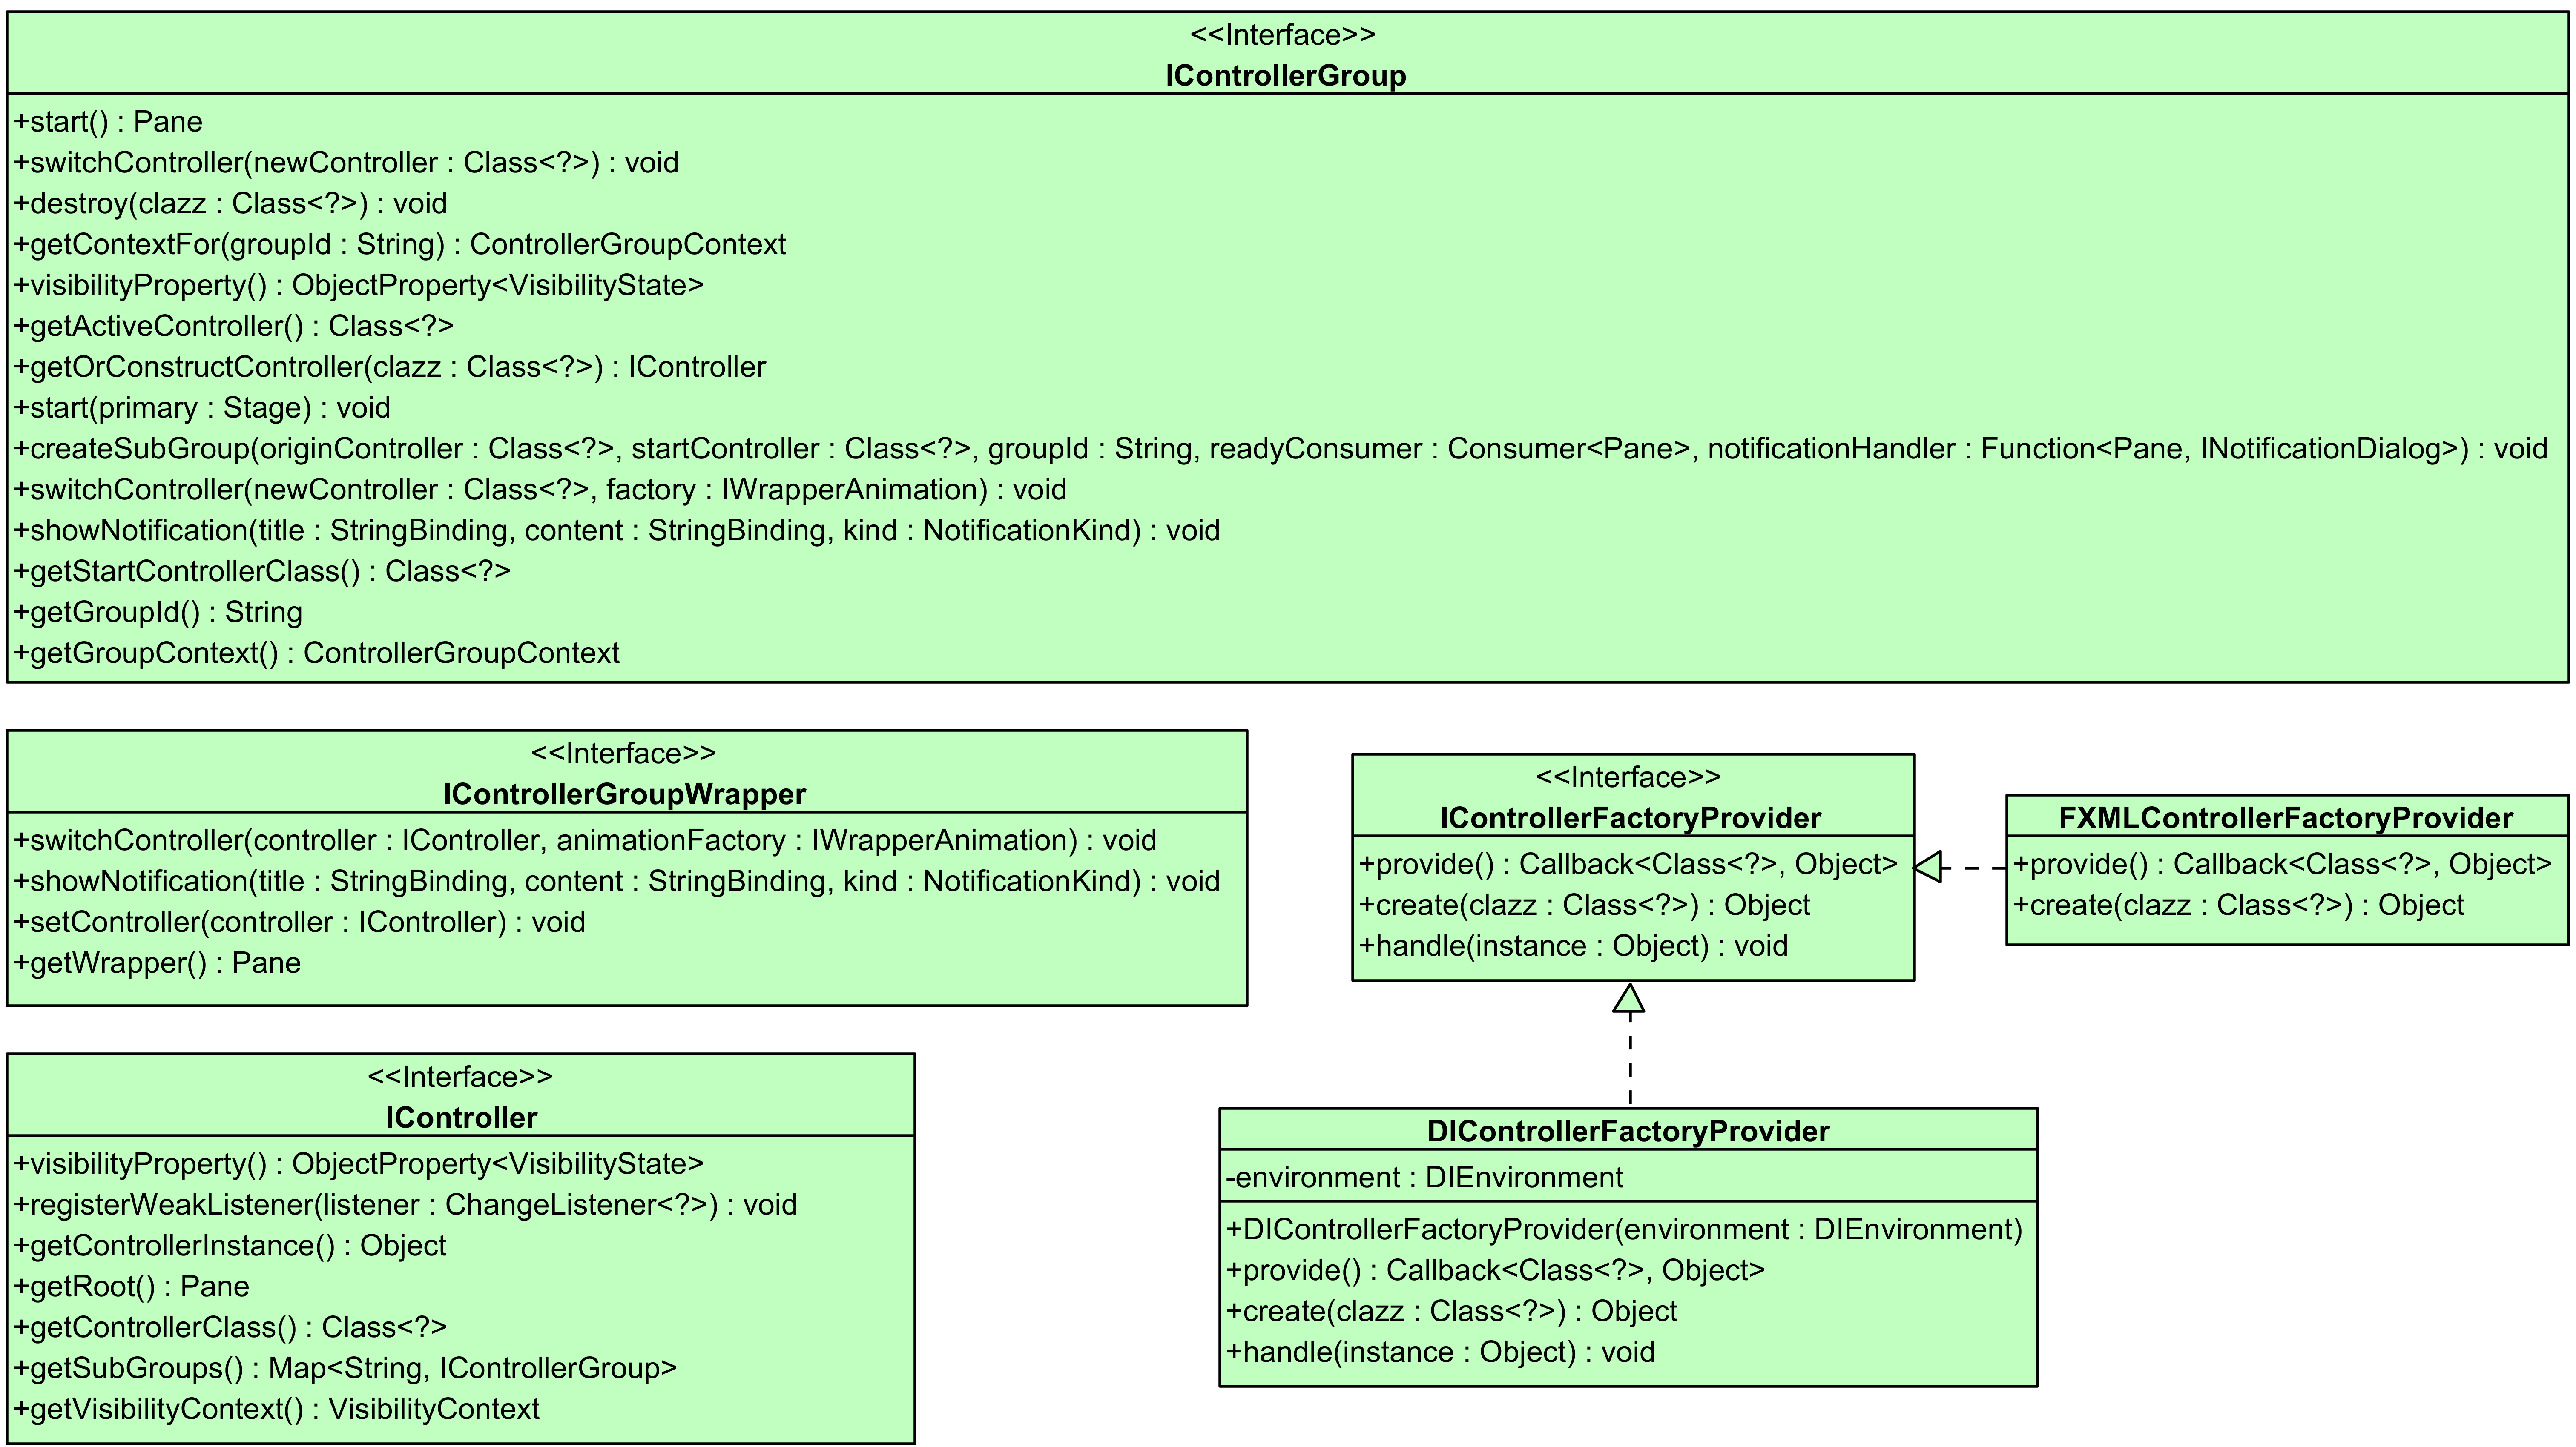
\includegraphics[angle=90,height=\textheight-2.2cm]{Abbildungen/Controller-System-Full.png}
	\caption*{Diagramm -- Controller-System: Einstiegspunkt und Beziehungen.}
\end{figure}
	\chapter{Demo Anwendung}
\label{appendix:demo_application}
\begin{figure}[H]
	\begin{lstlisting}[caption=Demo -- Minimaler Einstiegspunkt., captionpos=b, label=lst:entry_point_demo_full, numbers=left, xleftmargin=1.7em, framexleftmargin=1.7em, nolol]
#@StageConfig(title = "Login", icons = "icon.png")
#@ApplicationEntryPoint(MainController.class)
#@GuiceInjection(MainModule.class)
public final class DemoApplication {

    public static void main(String[] args) throws Exception {
        Reflection.addOpens("java.lang.reflect", "java.base",
				JFXTextFieldSkin.class.getModule());
        SimpliFX.launch();
    }

    #@ResourceBundle("lang.Messages")
    private II18N ii18N;

    #@ConfigSource("config/connection")
    private Properties properties;

    #@Shared
    private SharedReference<StringProperty> titleRef;

    #@EventHandler
    private void onStart(StartEvent event) {
        this.titleRef.set(event.getStage().titleProperty());
        event.getStage().show();
    }

}
	\end{lstlisting}
\end{figure}
\begin{figure}[H]
	\begin{lstlisting}[caption=Demo -- \texttt{MainController}., captionpos=b, label=lst:main_controller, numbers=left, xleftmargin=1.7em, framexleftmargin=1.7em, nolol]
#@Controller(fxml = "/fxml/MainController.fxml", 
#					 css = "css/main.css")
public final class MainController {

	#@FXML
	private BorderPane root;
	
	#@Setup
	private void setup(ControllerSetupContext ctx) {
		// Erstelle Untergruppe "titleBar" mit TitleBarController 
		// als Startcontroller
	    ctx.createSubGroup(TitleBarController.class, "titleBar", 
				this.root::setTop);
		// Erstelle Untergruppe "mainContent" mit LoginController
		// als Startcontroller
	    ctx.createSubGroup(LoginController.class, "mainContent",
				this.root::setCenter);
	}

}
	\end{lstlisting}
\end{figure}
\begin{figure}[H]
	\begin{lstlisting}[caption=Demo -- \texttt{LoginController}., captionpos=b, label=lst:login_controller, numbers=left, xleftmargin=1.7em, framexleftmargin=1.7em, nolol]
#@Controller(fxml = "/fxml/LoginController.fxml")
public final class LoginController {

	#@FXML
    private JFXTextField usernameField;

    #@FXML
    private JFXPasswordField passwordField;

    #@Shared
    private SharedReference<String> usernameRef;

    #@Shared
    private SharedReference<StringProperty> titleRef;

    #@Inject
    private ILoginService loginService;

    private ControllerGroupContext ctx;

    #@Setup
    private void setup(ControllerSetupContext ctx) {
        ctx.preloadController(MainMenuController.class);
        this.ctx = ctx.getGroupContext();
    }

    #@OnShow
    private void onShow() {
        this.titleRef.get().set("Login");
    }

    #@OnHide
    private void onHide() {
        this.usernameField.clear();
        this.passwordField.clear();
    }

    #@FXML
    private void onLogin() {
        if (loginService.login(this.usernameField.getText(),
				this.passwordField.getText())) {
            this.usernameRef.set(this.usernameField.getText());
            this.ctx.switchController(MainMenuController.class,
					new FadeAnimation(Duration.millis(250)));
        }
    }

}
	\end{lstlisting}
\end{figure}
\begin{figure}[H]
	\begin{lstlisting}[caption=Demo -- \texttt{MainMenuController}., captionpos=b, label=lst:mainmenu_controller, numbers=left, xleftmargin=1.7em, framexleftmargin=1.7em, nolol]
#@Controller(fxml = "/fxml/MainMenuController.fxml")
public final class MainMenuController {

    #@FXML
    private BorderPane root;

    #@FXML
    private StackPane contentCenter;

    #@ResourceBundle
    private II18N ii18N;

    #@Shared
    private SharedResources resources;

    private StringBinding binding;

    #@Setup
    private void setup(ControllerSetupContext ctx) {
        ctx.createSubGroup(SidebarController.class, "sidebar",
				this.root::setLeft);
        ctx.createSubGroup(TestControllerOne.class,
				"sidebarContent",
				this.contentCenter.getChildren()::setAll);
    }

    #@PostConstruct
    private void afterConstruction() {
        this.binding = this.ii18N
				.createObservedBinding("mainMenu.welcome",
						this.resources.getForName("username")
						.asProperty());
    }

    #@OnShow
    private void onShow() {
        final SharedReference<StringProperty> prop = 
				this.resources.getForName("title");
        prop.get().set(this.binding.get());
    }

}
	\end{lstlisting}
\end{figure}
\end{appendix}

% Abkürzungsverzeichnis
\include{Sonstiges/Abkürzungsverzeichnis}

% Codeverzeichnis
\lstlistoflistings

% Abbildungsverzeichnis
\listoffigures

% Tabellenverzeichnis
\listoftables

% Literaturverzeichnis...
\nocite{*}
\bibliographystyle{geralpha}
\bibliography{Bibliographie/Bibliographie}
%\listoftodos[Notes]

% Index ausgeben
\cleardoublepage
\addcontentsline{toc}{chapter}{Index}
\printindex

\end{document}
